\documentclass[]{book}
\usepackage{lmodern}
\usepackage{amssymb,amsmath}
\usepackage{ifxetex,ifluatex}
\usepackage{fixltx2e} % provides \textsubscript
\ifnum 0\ifxetex 1\fi\ifluatex 1\fi=0 % if pdftex
  \usepackage[T1]{fontenc}
  \usepackage[utf8]{inputenc}
\else % if luatex or xelatex
  \ifxetex
    \usepackage{mathspec}
  \else
    \usepackage{fontspec}
  \fi
  \defaultfontfeatures{Ligatures=TeX,Scale=MatchLowercase}
\fi
% use upquote if available, for straight quotes in verbatim environments
\IfFileExists{upquote.sty}{\usepackage{upquote}}{}
% use microtype if available
\IfFileExists{microtype.sty}{%
\usepackage{microtype}
\UseMicrotypeSet[protrusion]{basicmath} % disable protrusion for tt fonts
}{}
\usepackage[margin=1in]{geometry}
\usepackage{hyperref}
\PassOptionsToPackage{usenames,dvipsnames}{color} % color is loaded by hyperref
\hypersetup{unicode=true,
            pdftitle={National Wildlife Refuge Visitor Survey: Individual Refuge Results for Dungeness National Wildlife Refuge},
            pdfauthor={By Alia M. Dietsch, Colleen M. Hartel, Katie M. Lyon, and Natalie R. Sexton},
            colorlinks=true,
            linkcolor=Maroon,
            citecolor=Blue,
            urlcolor=Blue,
            breaklinks=true}
\urlstyle{same}  % don't use monospace font for urls
\usepackage{natbib}
\bibliographystyle{apalike}
\usepackage{longtable,booktabs}
\usepackage{graphicx,grffile}
\makeatletter
\def\maxwidth{\ifdim\Gin@nat@width>\linewidth\linewidth\else\Gin@nat@width\fi}
\def\maxheight{\ifdim\Gin@nat@height>\textheight\textheight\else\Gin@nat@height\fi}
\makeatother
% Scale images if necessary, so that they will not overflow the page
% margins by default, and it is still possible to overwrite the defaults
% using explicit options in \includegraphics[width, height, ...]{}
\setkeys{Gin}{width=\maxwidth,height=\maxheight,keepaspectratio}
\IfFileExists{parskip.sty}{%
\usepackage{parskip}
}{% else
\setlength{\parindent}{0pt}
\setlength{\parskip}{6pt plus 2pt minus 1pt}
}
\setlength{\emergencystretch}{3em}  % prevent overfull lines
\providecommand{\tightlist}{%
  \setlength{\itemsep}{0pt}\setlength{\parskip}{0pt}}
\setcounter{secnumdepth}{5}
% Redefines (sub)paragraphs to behave more like sections
\ifx\paragraph\undefined\else
\let\oldparagraph\paragraph
\renewcommand{\paragraph}[1]{\oldparagraph{#1}\mbox{}}
\fi
\ifx\subparagraph\undefined\else
\let\oldsubparagraph\subparagraph
\renewcommand{\subparagraph}[1]{\oldsubparagraph{#1}\mbox{}}
\fi

%%% Use protect on footnotes to avoid problems with footnotes in titles
\let\rmarkdownfootnote\footnote%
\def\footnote{\protect\rmarkdownfootnote}

%%% Change title format to be more compact
\usepackage{titling}

% Create subtitle command for use in maketitle
\providecommand{\subtitle}[1]{
  \posttitle{
    \begin{center}\large#1\end{center}
    }
}

\setlength{\droptitle}{-2em}

  \title{National Wildlife Refuge Visitor Survey: Individual Refuge Results for
Dungeness National Wildlife Refuge}
    \pretitle{\vspace{\droptitle}\centering\huge}
  \posttitle{\par}
    \author{By Alia M. Dietsch, Colleen M. Hartel, Katie M. Lyon, and Natalie R.
Sexton}
    \preauthor{\centering\large\emph}
  \postauthor{\par}
      \predate{\centering\large\emph}
  \postdate{\par}
    \date{2019-03-25}

\usepackage{booktabs}

% heading 4
\newcommand{\heading4}{
}
\usepackage{booktabs}
\usepackage{longtable}
\usepackage{array}
\usepackage{multirow}
\usepackage{wrapfig}
\usepackage{float}
\usepackage{colortbl}
\usepackage{pdflscape}
\usepackage{tabu}
\usepackage{threeparttable}
\usepackage{threeparttablex}
\usepackage[normalem]{ulem}
\usepackage{makecell}
\usepackage{xcolor}

\let\BeginKnitrBlock\begin \let\EndKnitrBlock\end
\begin{document}
\maketitle

{
\hypersetup{linkcolor=black}
\setcounter{tocdepth}{1}
\tableofcontents
}
\listoftables
\listoffigures
\chapter*{}\label{section}
\addcontentsline{toc}{chapter}{}

``Inspiring quote about the refuge lorem ipsum dolor sit amet,
consectetur adipiscing elit. Sed vestibulum lorem id purus laoreet, eget
luctus sem suscipit. In hac habitasse platea dictumst.''

---A visitor to Dungeness National Wildlife Refuge

\begin{center}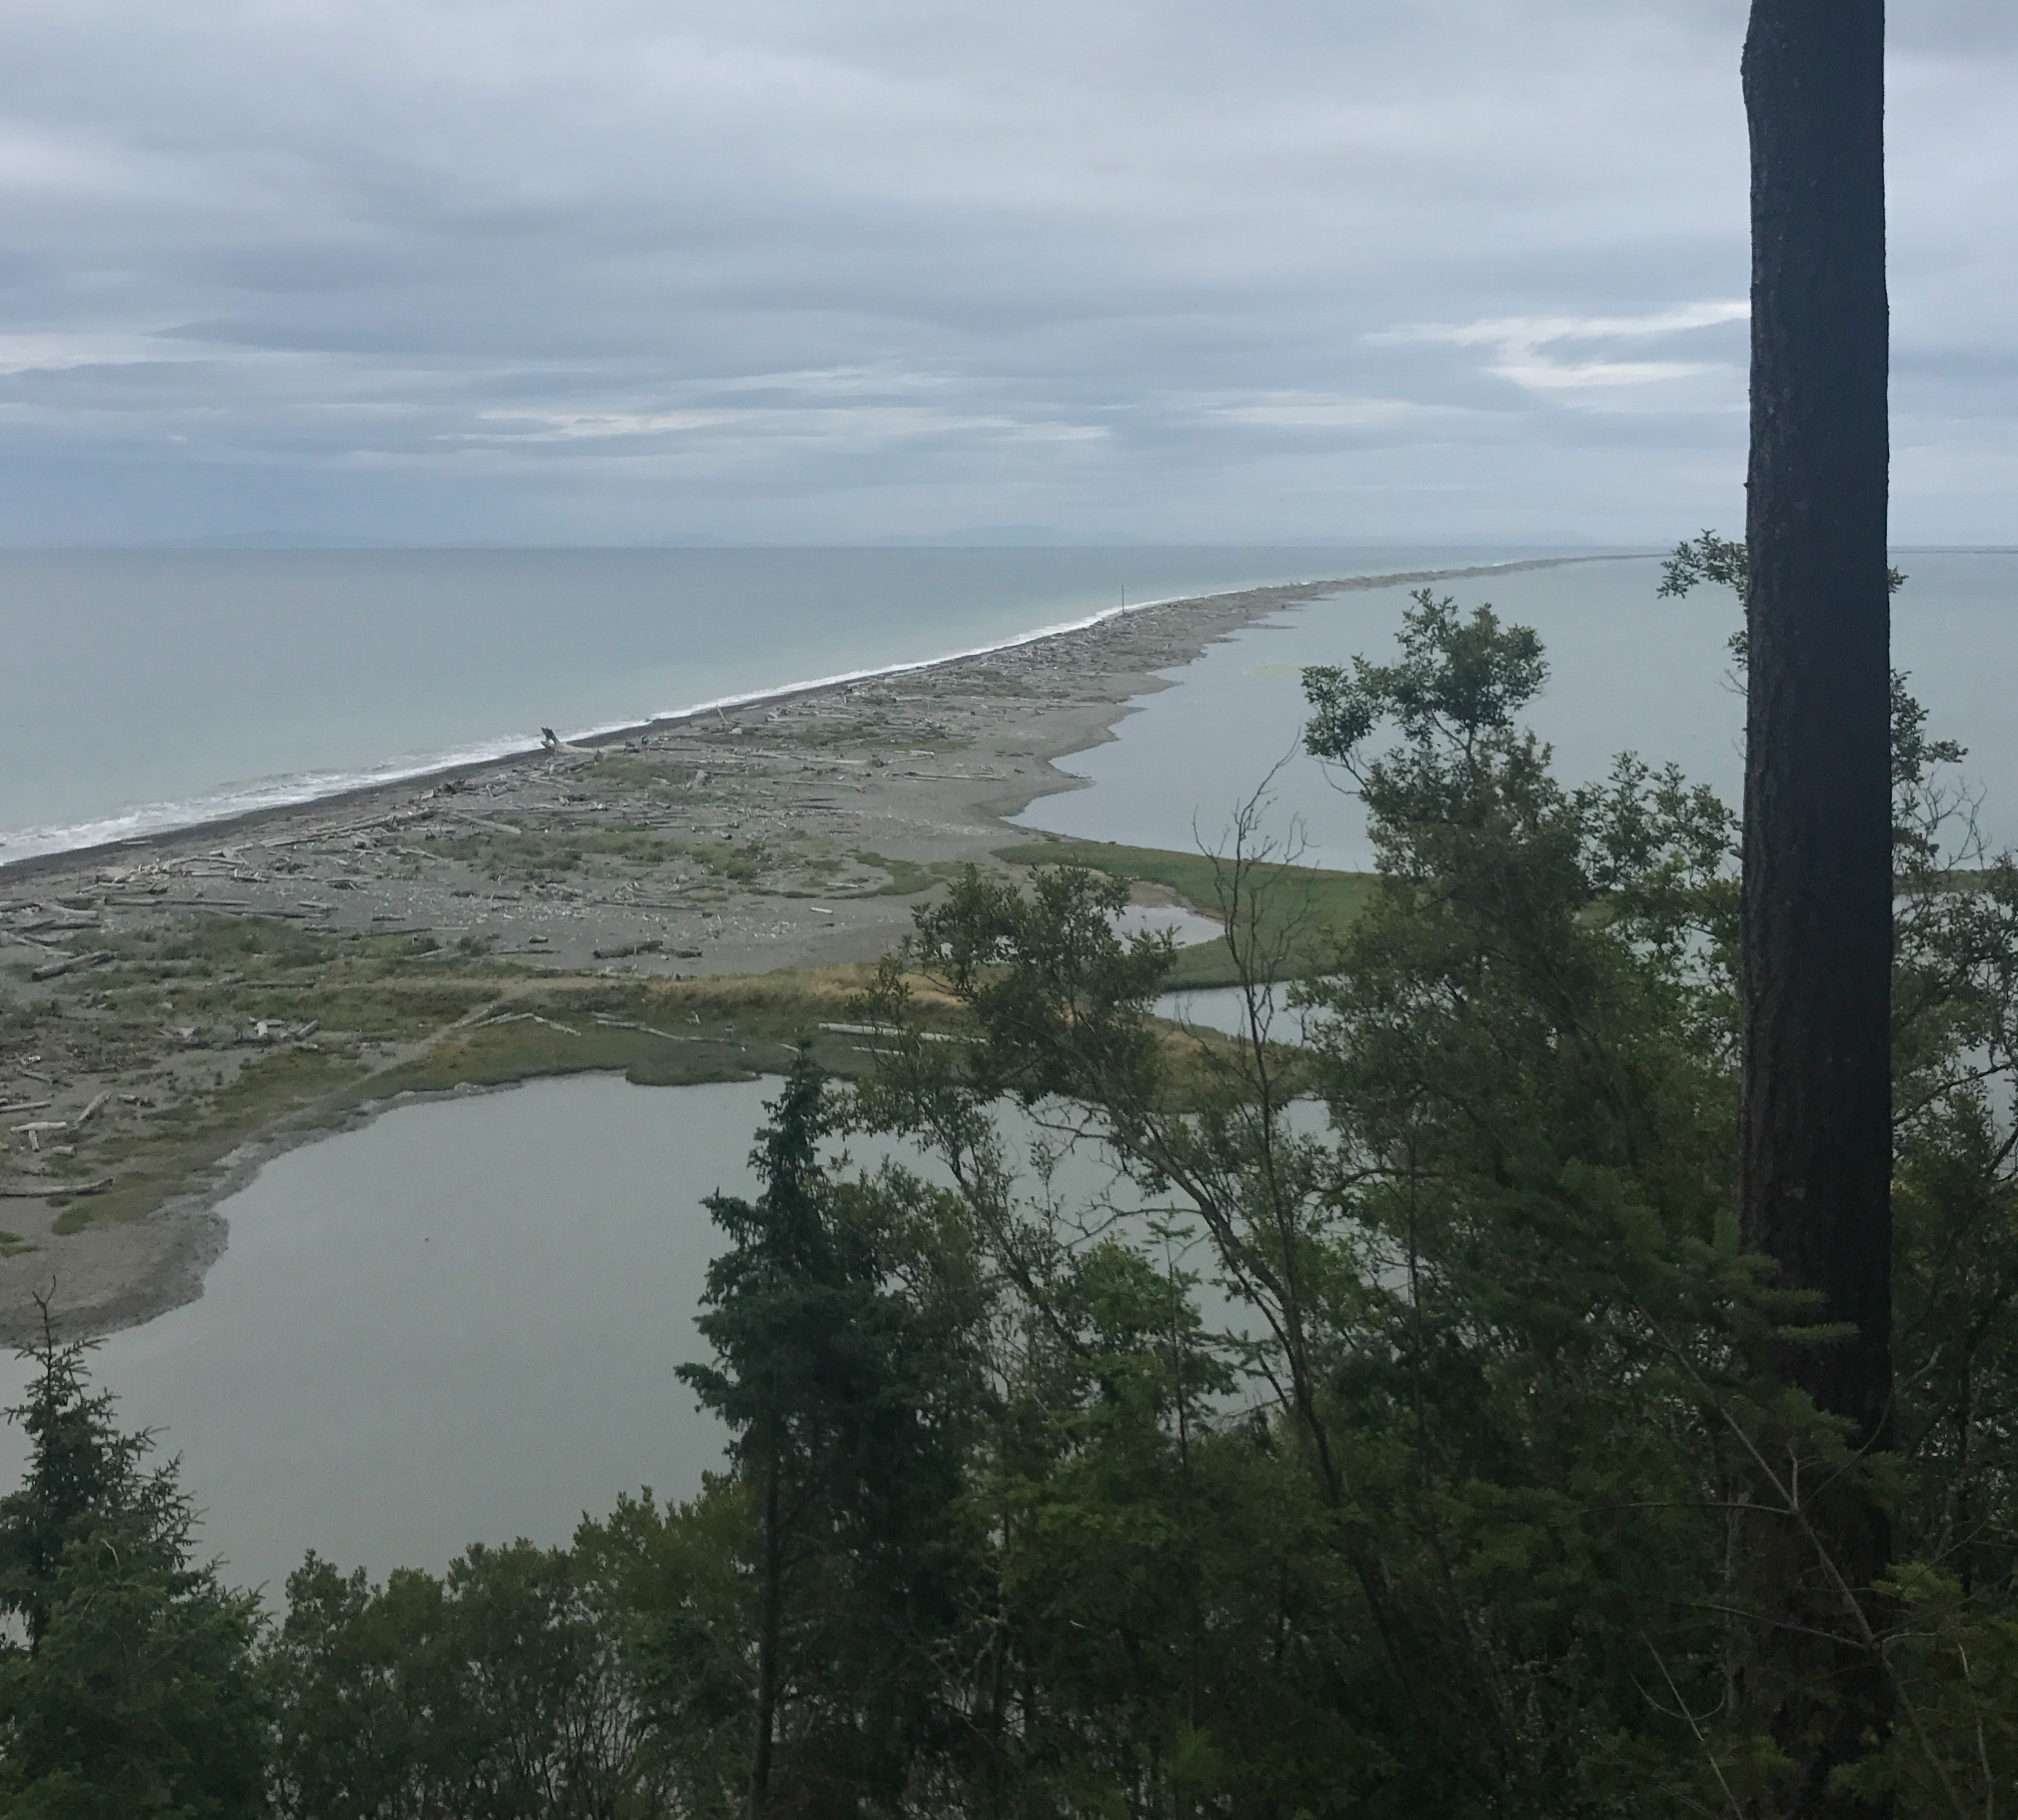
\includegraphics{refuge-info/Dungeness National Wildlife Refuge/cover} \end{center}

\chapter*{Acknowledgements}\label{acknowledgements}
\addcontentsline{toc}{chapter}{Acknowledgements}

This study was funded by the U.S. Fish and Wildlife Service's Natural
Resource Program Center, Division of Visitor Services and
Communications, and Transportation Program. The study design and survey
instrument were developed collaboratively with representatives from U.S.
Fish and Wildlife Service and researchers from The Ohio State University
(OSU). For their support and input to the study, we would like to thank
{[}names{]}; and any staff and volunteers at Dungeness National Wildlife
Refuge who assisted with the implementation of this survey effort.
Finally, we would like to especially acknowledge the following American
Conservation Experience team members for their work in implementing the
on-the-ground sampling for the 2018 survey effort: Ellen Bley, Kylie
Campbell, Michelle Ferguson, Justin Gole, James Puckett, Nicole Stagg,
and Angelica Varela. The success of this effort is largely a result of
their dedication to the project, as well as to the people who come to
explore these unique lands.

\textbf{Suggested citation:}

Dietsch, A. M., Hartel, C. M., Lyon, K. M., and Sexton, N.R. (2019).
``National Wildlife Refuge Visitor Survey: 2018 Individual Refuge
Results for Dungeness National Wildlife Refuge. The Ohio State
University, Columbus, OH.

\textbackslash{}begin\{figure\}

\{\centering 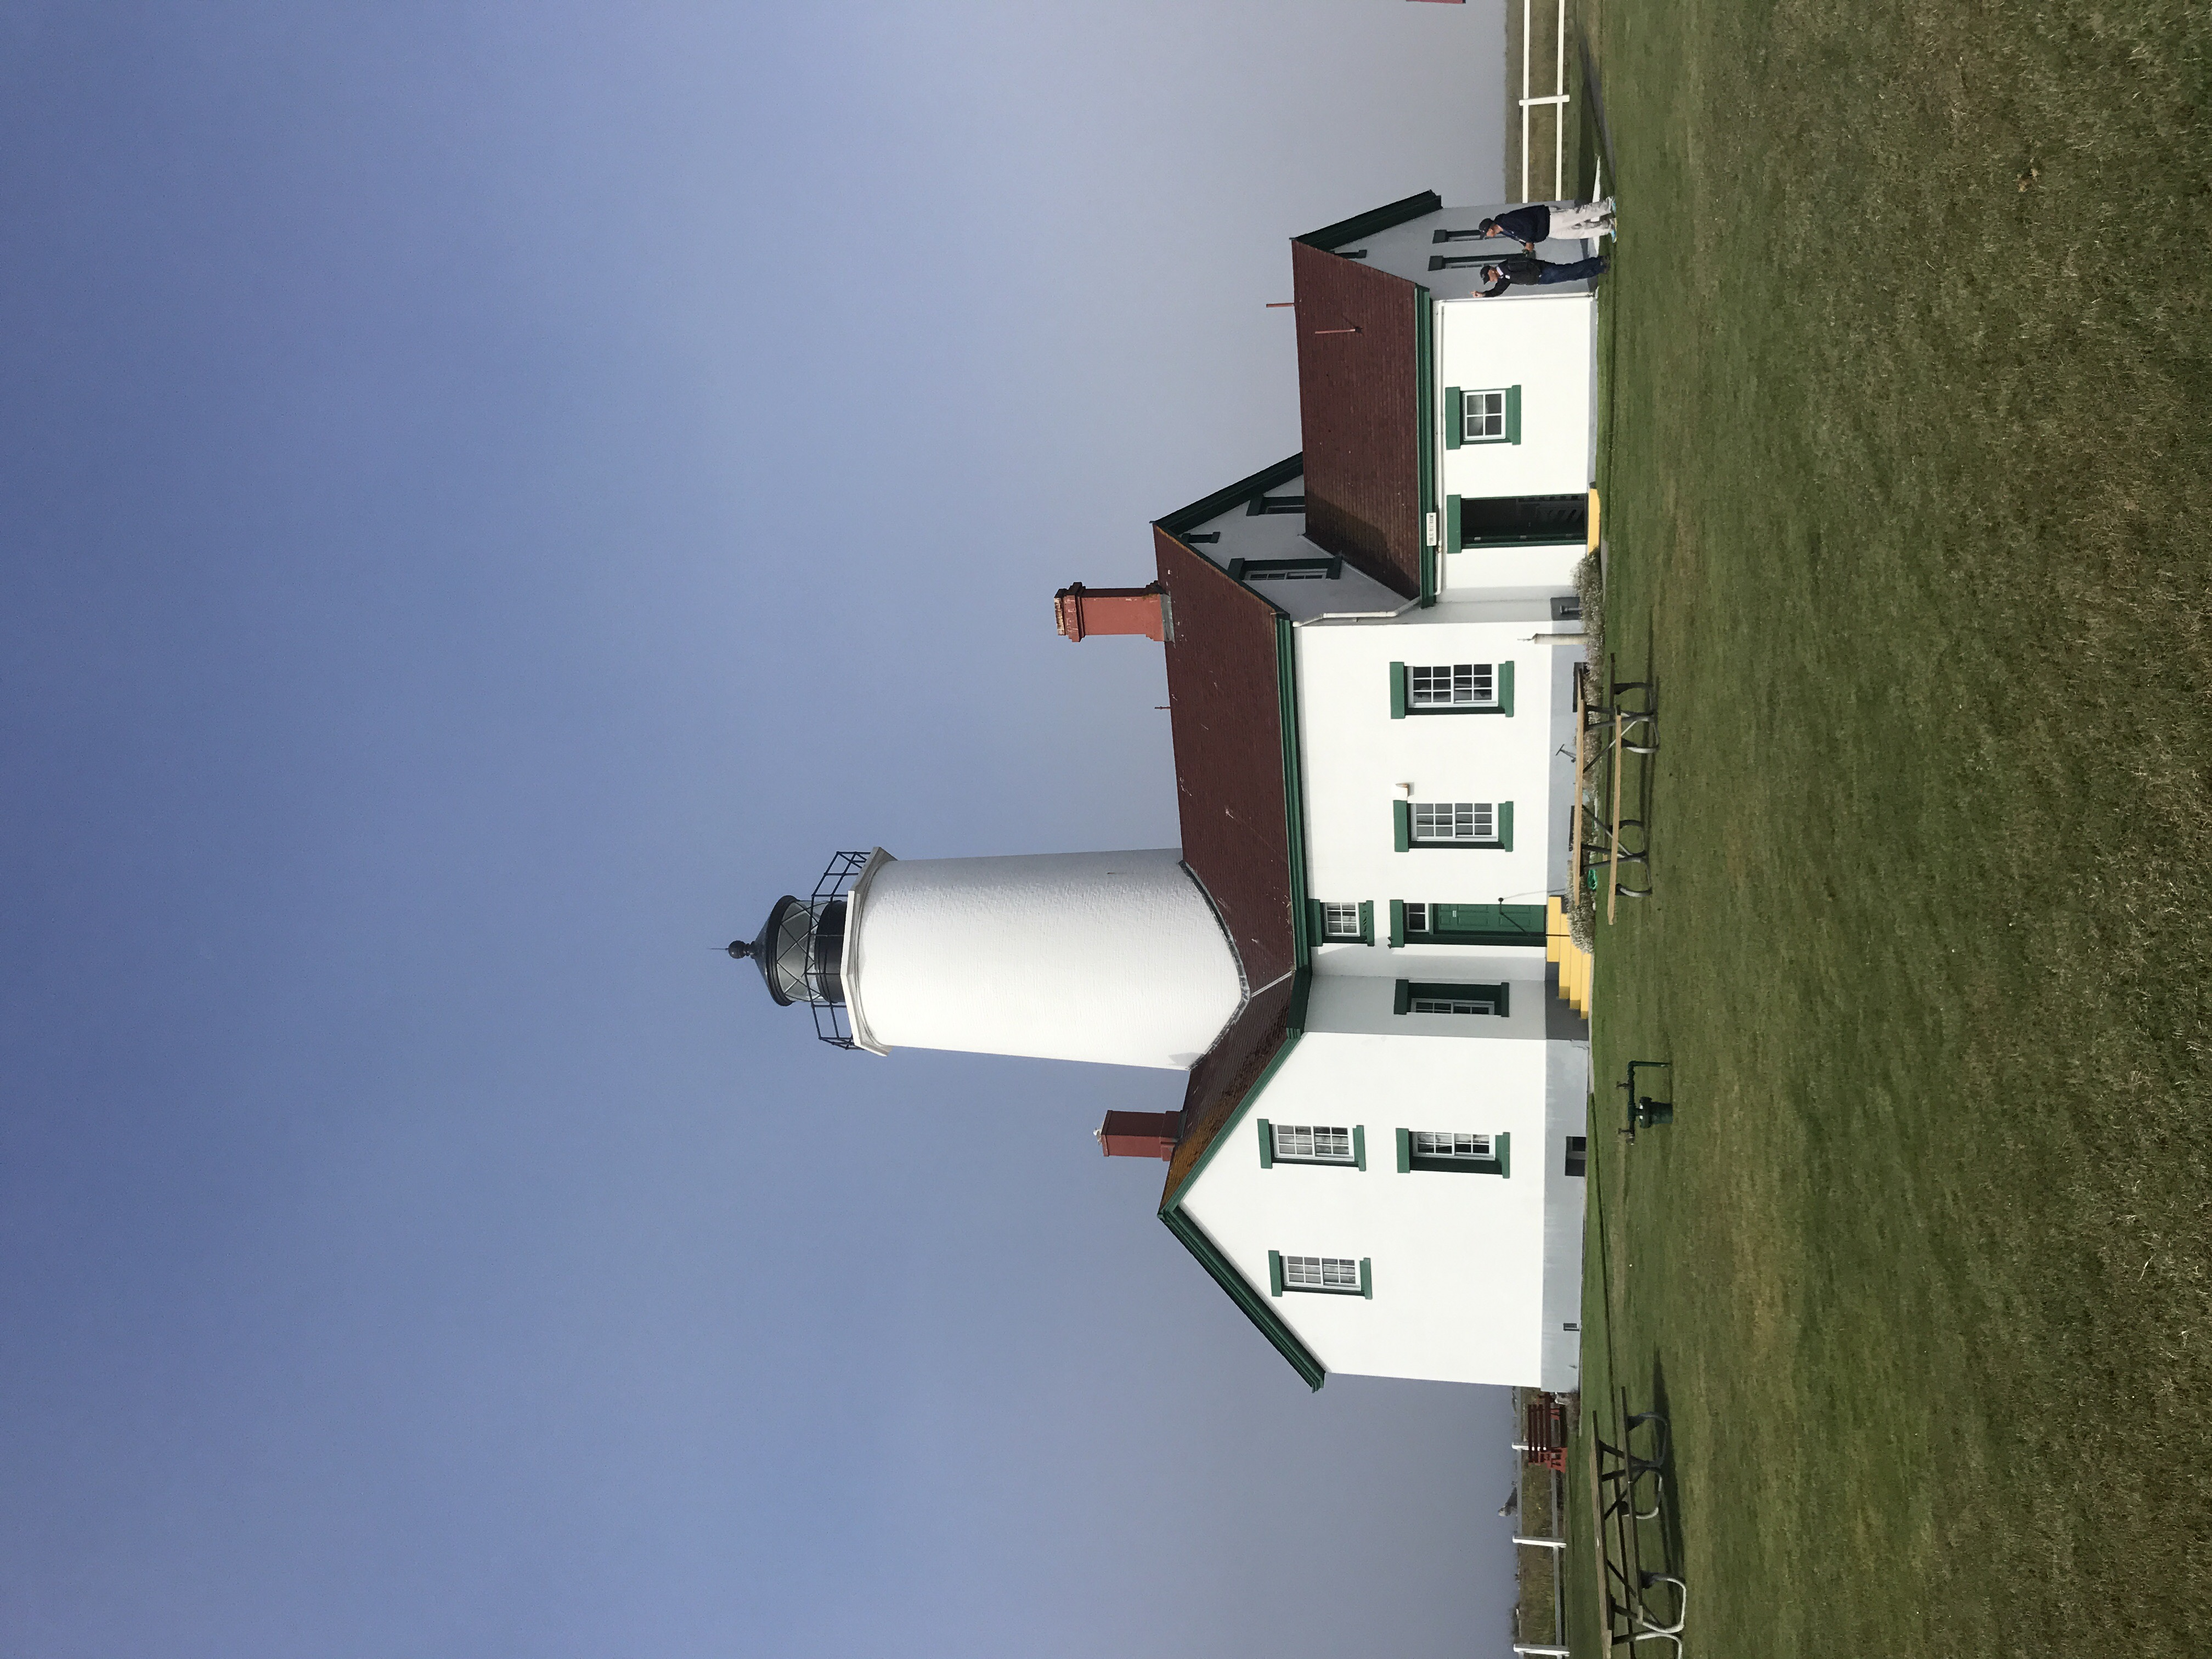
\includegraphics[width=42in,keepaspectratio]{refuge-info/Dungeness National Wildlife Refuge/image1}

\}

\textbackslash{}caption\{\texttt{r\ paste(\textquotesingle{}refuge-info\textquotesingle{},\ params\$RefugeName,\ \textquotesingle{}image1caption.txt\textquotesingle{},\ sep\ =\ \textquotesingle{}/\textquotesingle{})}\}\label{fig:ref-image1}
\textbackslash{}end\{figure\}

\chapter*{Executive Summary}\label{executive-summary}
\addcontentsline{toc}{chapter}{Executive Summary}

\section*{Overview}\label{overview}
\addcontentsline{toc}{section}{Overview}

This report describes the results of a visitor survey at Dungeness
National Wildlife Refuge (this refuge). Visitors were contacted during
two 2-week sampling periods to collect data on visitors' experiences. A
total of 291 visitor groups were contacted to participate in the survey.
Of those groups, 291 agreed to participate in the study. Questionnaires
were completed and returned by 291 visitors, resulting in a completion
rate of 1\% among those visitor groups that agreed to participate in the
study and an overall response rate of 1\% for the study.

The questions were designed to gather information on the following
themes:

\begin{itemize}
\tightlist
\item
  Activity participation and trip characteristics
\item
  Information sources used and their helpfulness
\item
  Modes of transportation used
\item
  Satisfaction with transportation, facilities, services, and recreation
  opportunties
\item
  Spending in the local area
\item
  Visitors opinions about this refuge
\item
  Transportation at this refuge
\item
  Visitor spending in the local communities
\item
  Enhancing future refuge visits
\end{itemize}

\textbf{Key Findings:}

\begin{itemize}
\tightlist
\item
  Hiking/Walking is the most commonly mentioned primary reason for
  visiting (30\%)
\item
  11\% respondents had visited the refuge before
\item
  Visitors average \texttt{r} visits per year
\item
  Visit length averages \texttt{r} hours
\item
  The most frequently used information resource is personal knowledge
  from previous visits (86\%). Other frequently used information sources
  are Refuge employees or volunteers (72\%) and Kiosks/displays/exhibits
  at this refuge (68\%). More than \texttt{r} (\texttt{r}\%) did not
  obtain any outside information prior to visiting.
\end{itemize}

\chapter{Introduction}\label{intro}

The National Wildlife Refuge System plays a unique role in connecting
current and future generations to our nation's rich natural heritage. A
national wildlife refuge visit can instill a lasting passion for
wildlife and wild lands. A carefully designed set of amenities,
services, and recreational opportunities contributes to and enhances the
visitor experience, making these important connections possible.
Opportunities for outdoor recreation draw millions of people each year
to national wildlife refuges. Many visitors enjoy hiking, paddling,
wildlife viewing or nature photography. Others take part in heritage
sports such as hunting and fishing. All these activities offer visitors
a chance to unplug from the stresses of modern life and reconnect with
their natural surroundings.

\section*{The National Wildlife Refuge
System}\label{the-national-wildlife-refuge-system}
\addcontentsline{toc}{section}{The National Wildlife Refuge System}

Established in 1903, and managed by the U.S. Fish and Wildlife Service
(Service), The National Wildlife Refuge System (Refuge System) is the
leading network of protected lands and waters in the world specifically
dedicated to the conservation of fish, wildlife, and their habitats.
With 55 million visits per year, the Refuge System is committed to
maintaining customer satisfaction and public engagement and strives to
be the best place for people and wildlife to thrive \citep{USFWS2018}.

As stated in the National Wildlife Refuge Improvement Act of 1997, the
mission of the Refuge System is ``to administer a national network of
lands and waters for the conservation, management and, where
appropriate, restoration of the fish, wildlife, and plant resources and
their habitats within the United States for the benefit of present and
future generations of Americans.'' Part of achieving this mission is the
goal ``to foster understanding and instill appreciation of the diversity
and interconnectedness of fish, wildlife, and plants, and their
habitats'' and ``to provide and enhance opportunities to participate in
compatible wildlife-dependent recreation.'' There are 567 national
wildlife refuges (refuges) and 38 wetland management districts
nationwide, including possessions and territories in the Pacific and
Caribbean, encompassing 95 million acres of land \citep{USFWS2018}.
(QUESTION: Do we add marine national monuments and submerged lands and
waters?) There is at least one refuge in every state and territory and
within an hour's drive of most major cities. This accessibility makes it
easy for communities to enjoy their wildlife heritage. The Refuge System
attracts more than 55 million visitors annually, including 39.6 million
people who observe and photograph birds and wildlife, 9.7 million who
hunt and fish, and 2.6 million teachers and students who use refuges as
outdoor classrooms.

\section*{Why a survey of refuge
visitors?}\label{why-a-survey-of-refuge-visitors}
\addcontentsline{toc}{section}{Why a survey of refuge visitors?}

Understanding visitor perceptions of refuges and characterizing their
experiences on refuges are critical elements of managing refuges and
meeting the goals of the Refuge System. The President's Management
Agenda identifies the National Wildlife Refuge System as a high-impact
service provider. Refuges work to maintain a high level of customer
satisfaction by operating visitor centers; designing, installing and
maintaining accessible trails; constructing viewing blinds; issuing
special use permits; contracting with private concessions, and
leveraging low recreation fees for facility improvements.

Understanding changing visitor trends requires the same commitment to
robust inventory and monitoring that the Refuge System has so diligently
applied throughout its history. The national visitor survey effort
provides managers, planners, visitor services specialists, and others
with reliable baseline data. Knowing who visits refuges and what they
do, how satisfied they are with their experience, and what their
economic contributions are to the local community help refuge staff
communicate the value of the refuge, set priorities, plan better, and
track trends over time.

The purpose of the overall effort is to better understand visitor
experiences and trip characteristics on refuges across Refuge System, to
gauge visitors levels of satisfaction with existing recreational
opportunities, and to garner feedback from visitors about their trips to
inform the design of programs and facilities. The survey results are
intended to inform performance, planning, budget, and communications
goals. Results will also inform Comprehensive Conservation Plans (CCPs),
visitor services, and transportation planning processes. Baseline
information is also fundamental to the Service's Inventory and
Monitoring Initiative, and can be used to assess changes over time
\citep{USFWS2017}.

Systematic monitoring of national wildlife refuges with 50,000 or more
visitors per year will occur on a 5-year rotating basis (approx. 36
refuges/year). Visitors are contacted onsite, and the survey is
administered by mail (with web option) once visitors return home.

The national visitor survey is a collaborative effort between the
Service, The Ohio State University (OSU), and American Conservation
Experience (ACE).

\chapter{Refuge Description}\label{refuge-description}

Dungeness NWR is located on the Olympic Peninsula in Sequim, WA. The
refuge was established in 1915 to preserve the unique habitat of the
Dungeness Spit, the longest natural sand spit in the United States. The
gravel beaches of the spit and the surrounding tide flats, eel beds, and
bay provide habitat and nesting ground for a variety of birds and other
species. While the refuge is only 773 acres, many different migratory
species use the refuge seasonally while others call it home year round.
Shorebirds migrate to the refuge in the spring and fall to feed in the
highly productive tide flats and waterfowl spend their winters in the
calm waters of the Dungeness Bay. Perhaps the most charismatic wildlife
to call the refuge home are harbor seals who raise their pups on the
isolated tip of the spit. Young salmon and steelhead feed and grow in
the eelgrass beds surrounding the spit. In addition, the second oldest
lighthouse in the state of Washington still shines bright on the refuge.
Built in 1857, the lighthouse is a popular hiking destination. The spit
continues to grow each year as the sandy bluffs along the Washington
coast erode and are deposited along the spit.

Dungeness NWR attracts over 101,000 visitors annually (U.S. Fish and
Wildlife Service, 2018, written comm.). Visitors flock from around the
world to hike along this scenic beach. The 10 mile hike out and back to
the lighthouse is an exciting challenge for all ages, from eager Boy
Scouts to retirees. Along the beach, visitors can watch bald eagles soar
overhead and see flocks of gulls resting along the driftwood. Visiting
this refuge is often part of a trip to nearby Olympic National Park and
many visitors camp at the neighboring county park. Figure
\ref{fig:ref-map1} displays a map of Dungeness NWR. For more
information, please visit \url{https://www.fws.gov/refuge/Dungeness/}.

\textbackslash{}begin\{figure\}
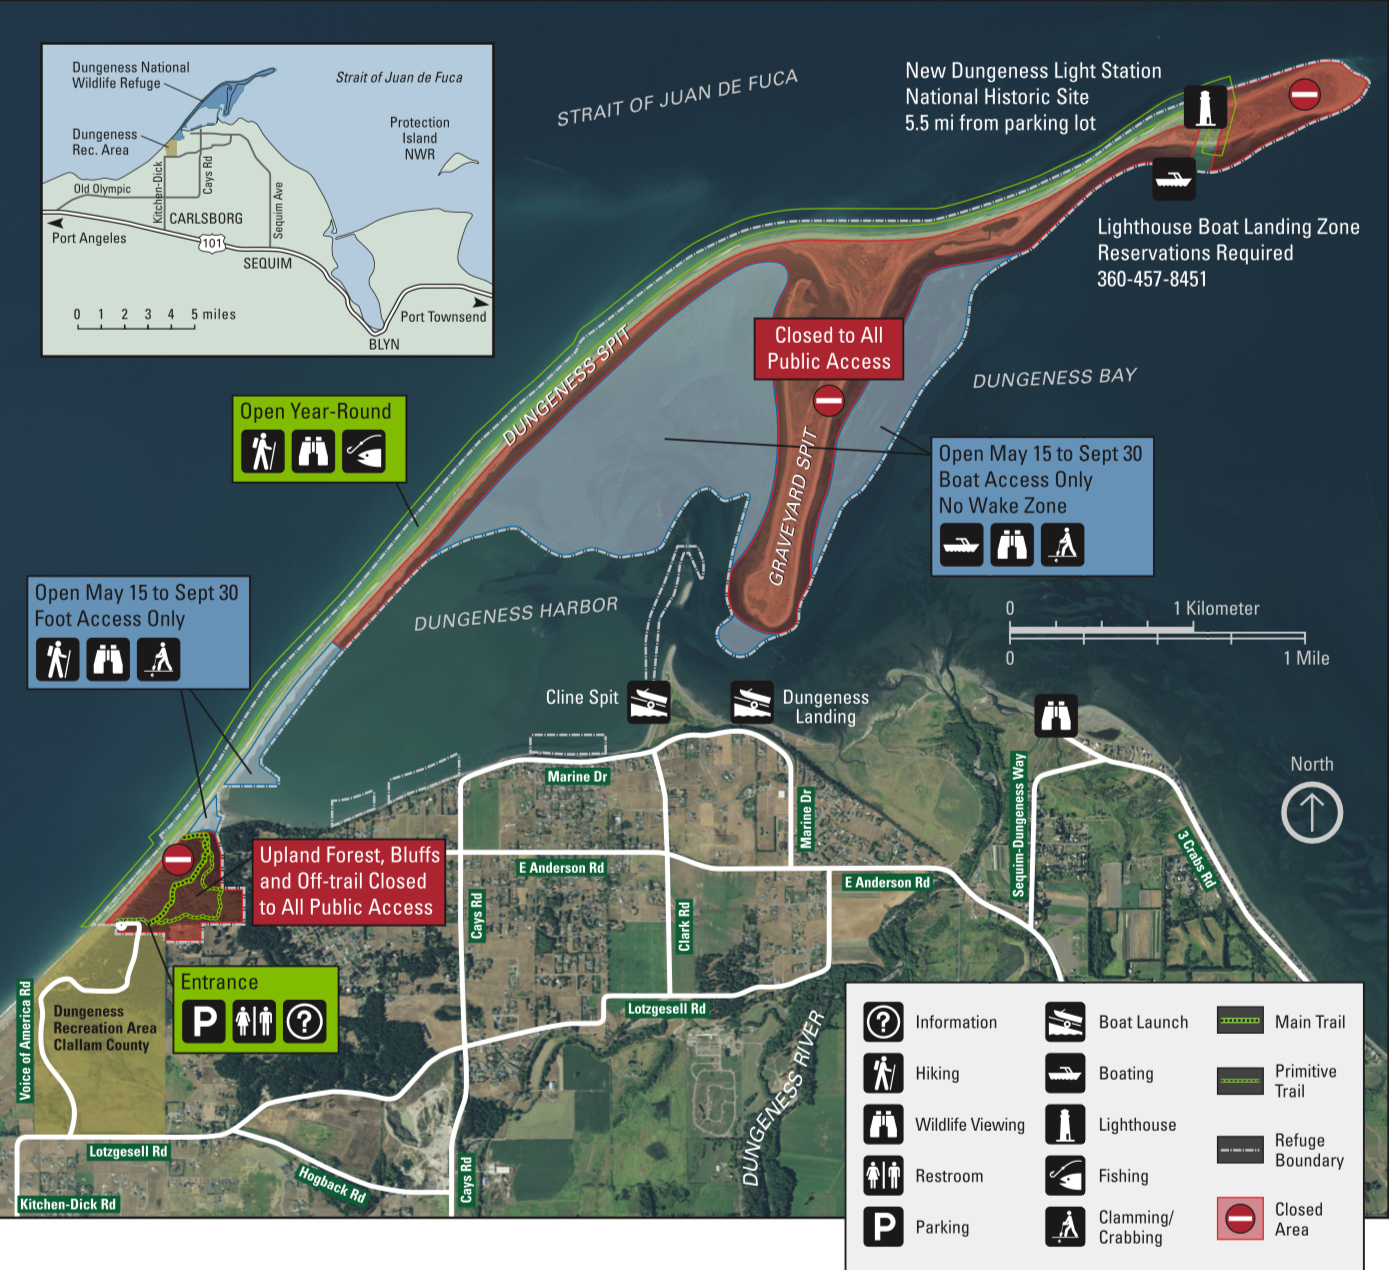
\includegraphics[width=19.29in]{refuge-info/Dungeness National Wildlife Refuge/map}
\textbackslash{}caption\{Map of
\texttt{params\$RefugeName}\}\label{fig:ref-map1}
\textbackslash{}end\{figure\} TODO: FIX CAPTION AND ADD MAP URL

\chapter{Methods}\label{methods}

\section*{Contacting Visitors}\label{contacting-visitors}
\addcontentsline{toc}{section}{Contacting Visitors}

Refuge staff identified two separate 14-day sampling periods, and one or
more locations at which to sample, that best reflected the diversity of
use and specific visitation patterns of each participating refuge. A
standardized sampling schedule was created for all refuges that included
eight randomly selected sampling shifts during each of the two sampling
periods. Sampling shifts were four hour time bands, stratified across AM
and PM as well as weekend and weekdays. In coordination with refuge
staff, any necessary customizations were made to the standardized
schedule to accommodate the identified sampling locations and to address
specific spatial and temporal patterns of visitation.

Twenty-five visitors (18 years of age or older) per sampling shift were
systematically selected, for a total of 375 willing participants per
refuge (or 200 per sampling period) to ensure an adequate sample of
completed surveys. When necessary, shifts were moved, added, or extended
to overcome logistical limitations (for example, weather or low
visitation at a particular site) in an effort to reach target numbers.

American Conservation Experience (ACE) interns and/or USFWS Human
Dimensions staff (survey recruiters) contacted visitors onsite following
a protocol provided by OSU that was designed to obtain a representative
sample. Instructions included contacting visitors across the entire
sampling shift (for example, every nth visitor for dense visitation, as
often as possible for sparse visitation) and contacting only one person
per group. Visitors were informed of the survey effort and asked to
participate. Willing participants provided their name, mailing address,
and preference for language (English or Spanish) and were given a small
token incentive (for example, a magnet or sticker) for their
participation. Survey recruiters were also instructed to record any
refusals and then proceed with the sampling protocol.

All visitors that agreed onsite to fill out a survey received the same
sequence of correspondence. This approach allowed for an assessment of
visitors' likelihood of completing the survey by their preferred survey
mode \citep{sexton2011}. Researchers at OSU sent the following materials
to all visitors agreeing to participate who had not yet completed a
survey at the time of each mailing \citep{dillman2014}:

\begin{itemize}
\tightlist
\item
  A postcard mailed within 10 days of the initial onsite contact
  thanking visitors for agreeing to participate in the survey and
  inviting them to complete the survey online.
\item
  A packet mailed 14 days later consisting of a cover letter, survey,
  and postage paid envelope for returning a completed paper survey.
\item
  A reminder postcard mailed 14 days later.
\item
  A second packet mailed 7 days later consisting of another cover
  letter, survey, and postage paid envelope for returning a completed
  paper survey.
\end{itemize}

Each mailing included instructions for completing the survey online, so
visitors had an opportunity to complete an online survey with each
mailing. Those visitors indicating a preference for Spanish were sent
Spanish versions of all correspondence (including the survey). Online
survey data were exported and paper survey data were entered into
Microsoft Excel using a standardized survey codebook and data entry
procedure. All survey data were analyzed using Statistical Package for
the Social Sciences (SPSS, v.23) software.\footnote{Any use of trade,
  firm, or product names is for descriptive purposes only and does not
  imply endorsement by the U.S. Government}

\section*{Sampling at This Refuge}\label{sampling-at-this-refuge}
\addcontentsline{toc}{section}{Sampling at This Refuge}

A total of 1 visitors agreed to participate in the survey during the two
sampling periods at the identified locations at Dungeness National
Wildlife Refuge Table \ref{tab:sampling-dates}. In all, 1 visitors
completed the survey for a 100\% response rate, and 10\% margin of error
at the 95\% confidence level.\footnote{A margin of error of ± 5\% at a
  95\% confidence level, for example, means that, if a reported
  percentage is 55\%, then 95 out of 100 times, that sample estimate
  would fall between 50\% and 60\% if the same question was asked in the
  same way. The margin of error is calculated with an 80/20 response
  distribution, assuming that for a given dichotomous choice question,
  approximately 80\% of respondents would select one choice and 20\%
  would select the other choice \citep{salant1994}.}

Table: \label{tab:sampling-dates}

\section*{Interpreting the Results}\label{interpreting-the-results}
\addcontentsline{toc}{section}{Interpreting the Results}

The extent to which these results accurately represent the total
population of visitors to this refuge is dependent on the number of
visitors who completed the survey (sample size) and the ability of the
variation resulting from that sample to reflect the beliefs and
interests of different visitor user groups \citep{scheaffer1996}. The
composition of the sample is dependent on the ability of the
standardized sampling protocol for this study to account for the spatial
and temporal patterns of visitor use unique to each refuge. Spatially,
the geographical layout and public-use infrastructure varies widely
across refuges. Some refuges can be accessed only through a single
entrance, while others have multiple unmonitored access points across
large expanses of land and water. As a result, the degree to which
sampling locations effectively captured spatial patterns of visitor use
will vary from refuge to refuge. Temporally, the two 14-day sampling
periods may not have effectively captured all of the predominant visitor
uses/activities on some refuges during the course of a year, which may
result in certain survey measures such as visitors' self-reported
``primary activity during their visit'' reflecting a seasonality bias.
Results contained within this report may not apply to visitors during
all times of the year or to visitors who did not visit the survey
locations.

In this report, visitors who responded to the survey are referred to
simply as ``visitors.'' However, when interpreting the results for
Dungeness National Wildlife Refuge, any potential spatial and temporal
sampling limitation specific to this refuge needs to be considered when
generalizing the results to the total population of visitors. For
example, a refuge that sampled during a special event (for example,
birding festival) held during the spring may have contacted a higher
percentage of visitors who traveled greater than 50 miles to get to the
refuge than the actual number of these people who would have visited
throughout the calendar year (that is, oversampling of nonlocals).
Another refuge may not have enough nonlocal visitors in the sample to
adequately represent the beliefs and opinions of that group type. If the
sample for a specific group type (for example, nonlocals, hunters,
visitors who paid a fee) is too low (n \textless{} 30), a warning is
included in the text. Finally, the term ``this visit'' is used to
reference the visit during which people were contacted to participate in
the survey.

\chapter{Visitor and Trip Characteristics}\label{visit}

Data collected as part of this survey provides a baseline from which to
understand who currently visits the refuge, and who engages in the
multitude of activities offered by the refuge. Baseline data also allow
refuge staff and others to assess any potential changes in visitor
characteristics over time, which is core to the scientific foundation of
the Service's Inventory and Monitoring Initiative \citep{USFWS2017}.

\section*{Visitor Characteristics}\label{visitor-characteristics}
\addcontentsline{toc}{section}{Visitor Characteristics}

\BeginKnitrBlock{heading4}
In particular, depictions of the demographics (e.g., age, economic
status, education, race and ethnicity) of both local and non-local
visitors can inform refuge managers about which groups of people are
directly benefitting from what the refuge currently offers. This type of
visitor data can then be compared with future visitor data to assess
changes in visitation due to various conditions (e.g., shifts in
climate, resource, staff, or infrastructure). Visitor demographics can
also be compared to the demographic composition of nearby communities
using data from U.S. Census, the American Community Survey, or through
online tools such as Social Explorer (www.socialexplorer.com) to assess
whether the nearby community composition is reflected within refuge
visitation, which is a critical component of getting to know and relate
to the community \citep{USFWS2014}. Such data can also determine what
new audiences from the local community - if not currently reflected in
the visitor population - could potentially be engaged through
appropriately-targeted outreach efforts (e.g., building partnerships,
enhancing stepping stones of engagement; \citep{USFWS2014}).
\EndKnitrBlock{heading4}

Visitors to Dungeness National Wildlife Refuge were 51\% male (with an
average age of 56 years) and 44\% female (with an average age of 54
years). Visitors, on average, reported they had 16 years of formal
education (equivalent to College). The median level of income was
\$50,000-\$74,999. See (AppendixB) for more demographic information.

\section*{Participation in Outdoor
Activities}\label{participation-in-outdoor-activities}
\addcontentsline{toc}{section}{Participation in Outdoor Activities}

\BeginKnitrBlock{heading4}
Quality recreational experiences on refuges provide opportunities for
visitors to connect with nature and the outdoors. Specifically,
wildlife-dependent recreation, such as hunting, fishing, wildlife
observation or photography, environmental education, and interpretation,
can increase visitor appreciation and knowledge of natural resources
\citep{USFWS2011}. The survey collected data on recreation participation
at this refuge during the past 12 months and the primary activity of
each visitor when they were contacted about the survey. Understanding
recreation participation can help to guide the allocation of resources,
including staff and infrastructure, to ensure visitors have quality,
memorable experiences. Understanding visitor uses of the refuge can also
aid in developing programs that facilitate meaningful interactions
between visitors and refuge staff. Finally, such information can also
help to pinpoint locations on the refuge where potential interactions
over refuge uses may be perceived as incompatible by different visitor
groups. Anticipating and preventing any social conflicts over refuge use
can help create a quality experience and foster personal and emotional
connections to the refuge and its resources \citep{USFWS2011}.
\EndKnitrBlock{heading4}

The most frequently participated in activities for all visitors were
Hiking/Walking (30\% of respondents), followed by Bird watching (17\% of
respondents). The primary activities reported at this refuge included:

\begin{itemize}
\tightlist
\item
  Hiking/Walking (30\%)
\item
  Bird watching (17\%)
\item
  Wildlife observation (13\%)
\end{itemize}

\begin{figure}
\centering
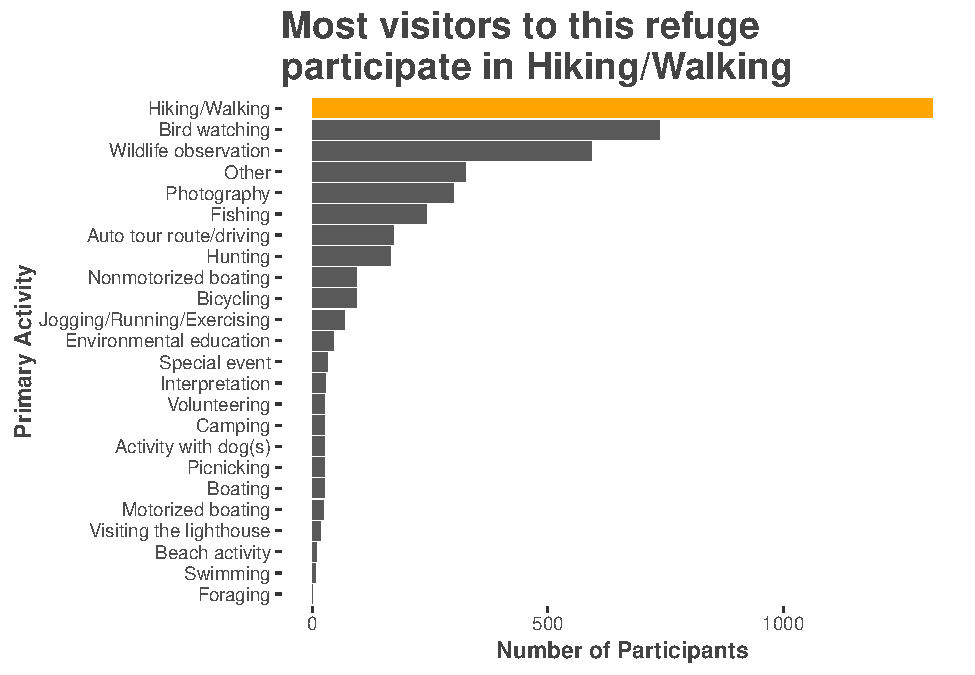
\includegraphics{nvs-report_files/figure-latex/primactFig-1.pdf}
\caption{\label{fig:primactFig}Primary activities}
\end{figure}

Refuge visitors were asked about twenty different activities they may
have participated in at this refuge during the 12 months prior to
completing the survey as well as the primary activity they participated
in during this visit. Frequencies of all twenty activities are included
in (AppendixB).

\begin{itemize}
\tightlist
\item
  Wildlife observation (74\%)
\item
  Hiking/Walking (69\%)
\item
  Bird watching (57\%)
\end{itemize}

Refuge visitors were also given the opportunity to write-in other
activities if they were not included in the list of twenty activities.
The full list of `other reported activities are included in (AppendixC).
Some of the unique activities reported at this refuge included:

\begin{itemize}
\tightlist
\item
  Wildlife observation (74\%)
\item
  Hiking/Walking (69\%)
\item
  Bird watching (57\%)
\end{itemize}

\section{Visiting This Refuge}\label{visiting-this-refuge}

\BeginKnitrBlock{heading4}
Understanding trends in overall visitation to this refuge provides
refuge staff with key information about its existing audiences.
Specifically, the survey explored the number of times visitors have been
to this refuge during the past year, including during which seasons, and
the trips taken to other refuges or other public lands for the same
primary activities. In combination with other trip characteristics
(e.g., trip purpose, time spent traveling to and visiting the refuge),
such information can be used to better understand activity and site
fidelity (i.e., likelihood of repeating specific past behavior) or
substitutability (i.e., likelihood of doing another activity or visiting
somewhere else to participate in a preferred activity). Such information
regarding site fidelity in particular can also help to identify the
success of existing communications at enticing different groups of
people to visit the refuge. Information on seasonality of visits can
help refuge staff anticipate when certain recreational activities or
programming is in high demand, an important informational need for
allocating appropriate resources.
\EndKnitrBlock{heading4}

Some of the key questions related to visitation habits to this refuge
included:

\begin{itemize}
\tightlist
\item
  Which of the following best describes your most recent visit to this
  refuge?
\end{itemize}

\subsection*{Group Composition}\label{group-composition}
\addcontentsline{toc}{subsection}{Group Composition}

Overall, 23\% of respondents indicated they were alone and 77\% of
respondents were with others on thier most recent visit to this refuge
(Table). On average, group size was 12.268873. The average group size
for localls was 3 and nonlocals was 3 (Table).

\subsection*{Visits to This Refuge and Other Public
Lands}\label{visits-to-this-refuge-and-other-public-lands}
\addcontentsline{toc}{subsection}{Visits to This Refuge and Other Public
Lands}

In the last 12 months, how many times have you visited this refuge
(including this visit)?

\begin{itemize}
\tightlist
\item
  35\% of visitors visited the refuge only once in the last 12 months
\item
  11\% of visitors visited the refuge two times in the last 12 months
\end{itemize}

\subsection*{Visits to other national wildlife
refuges}\label{visits-to-other-national-wildlife-refuges}
\addcontentsline{toc}{subsection}{Visits to other national wildlife
refuges}

In the last 12 months, how many times have you visited other national
wildlife refuges?

\begin{itemize}
\tightlist
\item
  74\% of visitors did not visit any other national wildlife refuges in
  the last 12 months
\item
  21\% of visitors visited other national wildlife refuges only once in
  the last 12 months
\item
  25\% of visitors visited other national wildlife refuges two times in
  the last 12 months
\end{itemize}

\subsection*{Visits to other public
lands}\label{visits-to-other-public-lands}
\addcontentsline{toc}{subsection}{Visits to other public lands}

In the last 12 months, how many times have you visited other public
lands (for example, national or state parks) to participate in the same
primary activity as this visit?

\begin{itemize}
\tightlist
\item
  28\% of visitors did not visit any other public lands
\item
  9\% of visitors visited other public lands only once
\item
  14\% of visitors visited other public lands two times
\end{itemize}

\subsection*{Travel to this refuge}\label{travel-to-this-refuge}
\addcontentsline{toc}{subsection}{Travel to this refuge}

\begin{itemize}
\tightlist
\item
  Approximately how many hours/minutes (one-way) did you travel from
  your home to this refuge?
\end{itemize}

\chapter{Communicating Refuge Information}\label{info}

\BeginKnitrBlock{heading4}
Effective communication with the public is critical for managing and
enhancing visitor experiences. Additionally, the Refuge System's success
in reaching new and diverse audiences depends on its ability to keep
pace with communication trends \citep{USFWS2016a}. Understanding how
visitors both seek out and share information about the refuge and its
resources using various communication channels (e.g., printed
information, friends and family, websites, social media) can inform the
refuge's approach to communicating with visitors at different points of
their trips (before, during and after). Information in this section can
be used to assess changes in what sources are used as well as how
visitors perceive the helpfulness of Service communications over time.
Refuge staff can use communication channels preferred by visitors to
inform the public about the Refuge System's mission and accomplishments.
\EndKnitrBlock{heading4}

\section*{Learning about This Refuge}\label{learning-about-this-refuge}
\addcontentsline{toc}{section}{Learning about This Refuge}

The survey asked which information sources visitors used to learn about
the refuge and its resources and the degree to which each information
source was helpful. Visitors across different ages may use different
information sources to learn about this refuge and its resources. The
full list of information sources presented to visitors is contained in
(AppendixB).

\hypertarget{left}{}
\subsection*{Learning about This
Refuge}\label{learning-about-this-refuge-1}
\addcontentsline{toc}{subsection}{Learning about This Refuge}

Visitors across different ages may use different information sources to
learn about this refuge and its resources. The full list of information
sources presented to visitors is contained in Appendix B.

Among all visitors, the following information sources were most
frequently rated as very or extremely helpful:

\begin{itemize}
\tightlist
\item
  Personal knowledge from previous visits (86\%)
\item
  Refuge employees or volunteers (72\%)
\item
  Kiosks/displays/exhibits at this refuge (68\%)
\end{itemize}

Visitors under the age of 35 most often used these information sources
to learn about the refuge:

\begin{itemize}
\tightlist
\item
  Personal knowledge from previous visits (80\%)
\item
  Web-based map (70\%)
\item
  Refuge employees or volunteers (67\%)
\end{itemize}

Visitors over the age of 35 most often used these information sources to
learn about the refuge:

\begin{itemize}
\tightlist
\item
  Personal knowledge from previous visits (87\%)
\item
  Refuge employees or volunteers (74\%)
\item
  Kiosks/displays/exhibits at this refuge (68\%)
\end{itemize}

\hypertarget{right}{}
\subsection*{Sharing Refuge
Experiences}\label{sharing-refuge-experiences}
\addcontentsline{toc}{subsection}{Sharing Refuge Experiences}

More than half of visitors (53\%) reported using social media to share
their refuge experience with other people. The full list of social media
outlets presented to visitors is contained in Appendix B.

Among all visitors, the following social media outlets were used most
often to share refuge experiences:

\begin{itemize}
\tightlist
\item
  None (47\%)
\item
  Facebook (39\%)
\item
  Instagram (14\%)
\end{itemize}

Visitors under the age of 35 most often used these social media outlets
to share refuge experiences:

\begin{itemize}
\tightlist
\item
  None (47\%)
\item
  Facebook (39\%)
\item
  Instagram (14\%)
\end{itemize}

Visitors over the age of 35 most often used these social media outlets
to share refuge experiences:

\begin{itemize}
\tightlist
\item
  None (47\%)
\item
  Facebook (39\%)
\item
  Instagram (14\%)
\end{itemize}

\section*{Helpfulness of Information
Sources}\label{helpfulness-of-information-sources}
\addcontentsline{toc}{section}{Helpfulness of Information Sources}

Among all visitors, the following information sources were most
frequently rated as very or extremely helpful:

\begin{itemize}
\tightlist
\item
  Personal knowledge from previous visits (86\%)
\item
  Refuge employees or volunteers (72\%)
\item
  Kiosks/displays/exhibits at this refuge (68\%)
\end{itemize}

Visitors under the age of 35 most often used these information sources
to learn about the refuge:

\begin{itemize}
\tightlist
\item
  Personal knowledge from previous visits (80\%)
\item
  Web-based map (70\%)
\item
  Refuge employees or volunteers (67\%)
\end{itemize}

Visitors over the age of 35 most often used these information sources to
learn about the refuge:

\begin{itemize}
\tightlist
\item
  Personal knowledge from previous visits (87\%)
\item
  Refuge employees or volunteers (74\%)
\item
  Kiosks/displays/exhibits at this refuge (68\%)
\end{itemize}

\chapter{Visitor Opinions about this Refuge}\label{opin}

\BeginKnitrBlock{heading4}
A baseline understanding of visitor experiences provides a framework
from which the Refuge System can monitor trends in visitor experiences
and opinions overtime. Obtaining such a baseline is integral to the
Service's Inventory and Monitoring Initiative \citep{USFWS2017}, as well
as warranted if the Service is to remain relevant in the face of
changing demographics and wildlife-related interests \citep{USFWS2014}.
As part of the survey, visitors rated both the importance of different
serv, facilities, and opportunities on the refuge, and their
satisfaction with each of the things applicable to their refuge
experience. Certain services or recreational opportunities may be more
or less central to the experience of different segments of the visitor
population, and the potential for highly varied importance ratings needs
to be considered when viewing the satisfaction results of this analysis.
For example, hunters may place more importance on hunting opportunities
and amenities, while school-group leaders may place more importance on
educational/informational displays. Thus, a specialized user group's
importance of and satisfaction with a particular attribute may differ
from the overall importance of and satisfaction with that same attribute
for the full sample of visitors summarized in this report.
\EndKnitrBlock{heading4}

\section*{Overall Satisfaction}\label{overall-satisfaction}
\addcontentsline{toc}{section}{Overall Satisfaction}

The vast majority of surveyed visitors were satisfied with the refuge's
job of conserving fish, wildlife, and their habitats (83\%) and the
quality of the overall experience when visiting this refuge (87\%). The
next step is to compare the importance and satisfaction ratings for
visitor services provided by refuges in order to identify how well
different services meet visitor expectations.

\section*{Services and Facilities}\label{services-and-facilities}
\addcontentsline{toc}{section}{Services and Facilities}

Positive experiences are driven by first impressions of refuge
facilities and people.

\section*{Recreational Opportunities}\label{recreational-opportunities}
\addcontentsline{toc}{section}{Recreational Opportunities}

\section*{Feeling Safe and Welcome}\label{feeling-safe-and-welcome}
\addcontentsline{toc}{section}{Feeling Safe and Welcome}

\BeginKnitrBlock{heading4}
People who rarely participate in wildlife-dependent recreation or do not
regularly visit refuges may have different perspectives on the role of a
refuge and its resources in everyday life compared to people who
regularly visit a refuge or frequently participate in wildlife-dependent
recreation. Visitors, particularly those new to `being in nature', may
have a sense of danger when outdoors or general discomfort associated
with the unknown \citep{USFWS2014}. Additionally, some people may
perceive the refuge to lack materials or programs accessible and
relevant to their interests, or may even believe that natural places are
unwelcoming because of historical associations with the outdoors. Thus,
an understanding of how visitors rate their feelings of being safe and
welcome on the refuge can provide important baseline information to
refuge staff when identifying potential areas for improvement and
evaluating how future efforts may enhance feelings of being safe and
welcome at refuges over time.
\EndKnitrBlock{heading4}

\chapter{Transportation at this Refuge}\label{trans}

\BeginKnitrBlock{heading4}
Transportation networks connect local communities to refuges and are the
bedrock of all experiences that occur on refuges. Visitors access
refuges by car, by boat, by bike, and by plane. The Service works to
ensure that the roads, trails and parking areas are welcoming and safe
for visitors of all abilities.These networks include roads, bridges,
foot pathways, entrances, and the entire suite of transportation
features critical to visitor access and mobility. While many visitors
arrive at the refuge in private vehicles, other options (including
buses, trams, watercraft, and bicycles) are increasingly becoming a part
of the visitor experience. Thus, there is a critical need to know how
visitors perceive the safety of using these different transportation
options, as well as different transportation features (e.g., bridges,
roadways, entrances/exists) as part of their experience. The survey
asked visitors to rate both the importance and current satisfaction with
existing transportation-related features, as well as methods of
transportation visitors used to get to and around the refuge during
their visit. This information can help to identify if transportation
improvements could be made that would further enhance visitor access
and, ultimately, their overall experiences \citep{USFWS2011}.
Additionally, transportation alternatives within the Refuge System
\citep{krechmer2001, volpe2010} could help to improve refuge conditions
(e.g., quality of air, water, and habitat); thus, the survey asked
visitors to note different transportation methods used during their
trips, and their likelihood of using alternative transportation at
refuges in the future.
\EndKnitrBlock{heading4}

\section*{Travel To This Refuge}\label{travel-to-this-refuge-1}
\addcontentsline{toc}{section}{Travel To This Refuge}

The key mode of transportation used by visitors to travel to this refuge
was Private vehicle without trailer (86\%; fig. 11). The key mode of
transportation used by visitors to travel around this refuge was Foot
(46\%).

\textbf{Figure 11.} Modes of transportation used by visitors to travel
to and around Dungeness National Wildlife Refuge during this visit
(\emph{n} = \#\#\#). See Appendix C for a listing of ``other'' modes of
transportation. Modes of transportation with a proportion smaller than
1.5\% for both items were excluded; see Appendix B for frequencies of
all items.

\section*{Transportation-related
Features}\label{transportation-related-features}
\addcontentsline{toc}{section}{Transportation-related Features}

A majority of visitors to Dungeness National Wildlife Refuge thought
transportation-related items were important Figure \ref{fig:trans-imp}.
They were most satisfied with x and least satisfied with y Figure
\ref{fig:trans-sat}.

\begin{figure}
\centering
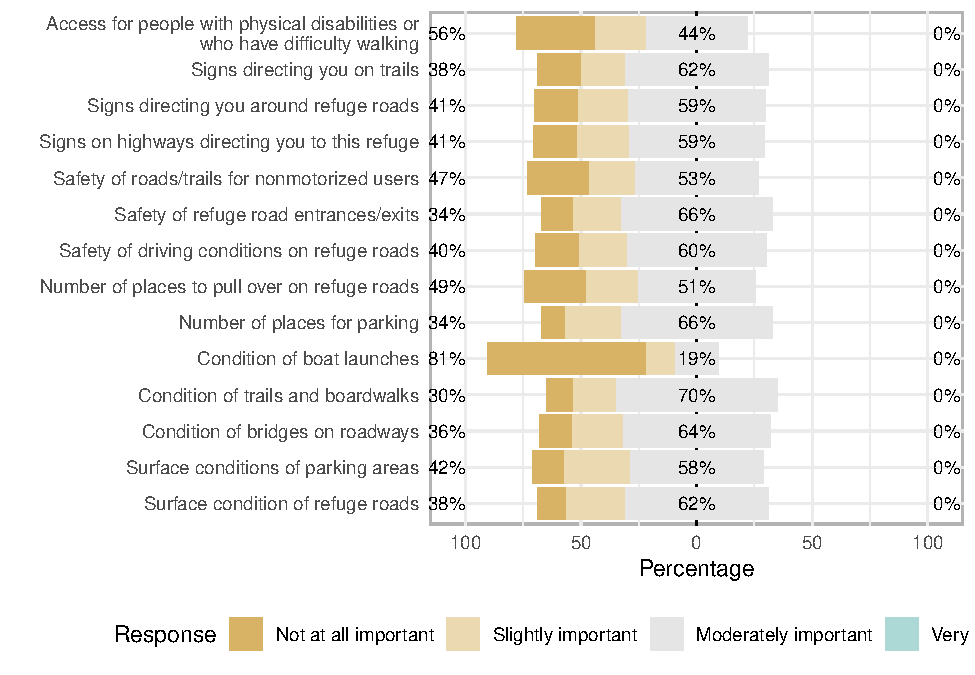
\includegraphics{nvs-report_files/figure-latex/trans-imp-1.pdf}
\caption{\label{fig:trans-imp}Importance of transportation-related features
when visiting this refuge}
\end{figure}

\begin{figure}
\centering
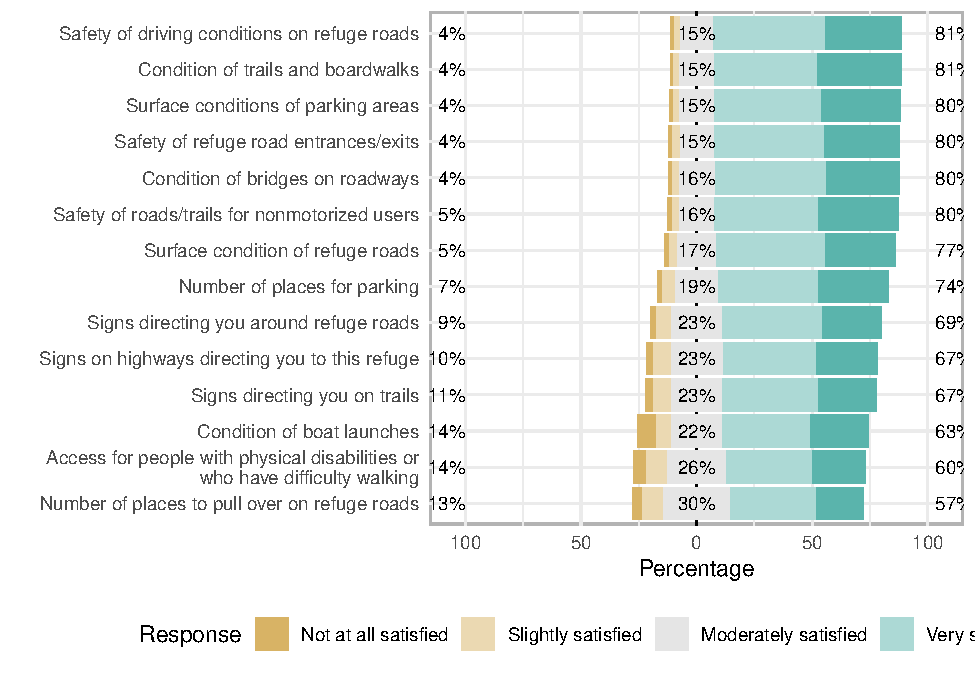
\includegraphics{nvs-report_files/figure-latex/trans-sat-1.pdf}
\caption{\label{fig:trans-sat}Rate how satisfied you are with the way this
refuge is managing each feature}
\end{figure}

\section*{Alternative Transportation
Options}\label{alternative-transportation-options}
\addcontentsline{toc}{section}{Alternative Transportation Options}

One goal of the Transportation Program is to provide alternative modes
and means of access to FWS managed lands as a way to enhance the
visitation experience. ``Access to FWS managed lands, where compatible
with Station purpose, should be available to visitors via multiple forms
of transportation, including public transit, bicycle, and walking.
Alternative forms of transportation can help reduce visitors' carbon
footprints, which in turn may have long term positive affects for the
natural resources we manage. Planning and building to accommodate
sustainable transportation options can help to achieve the FWS mission
\citep{USFWS2016b}.

Of six alternative transportation options listed on the survey, a
majority of refuge visitors were likely to use the following at
Dungeness National Wildlife Refuge in the future Figure
\ref{fig:alt-trans}:

\begin{itemize}
\tightlist
\item
  Pedestrian paths for access to this refuge from the local community
  (23\%)
\item
  Bus or tram that provides a guided tour (15\%)
\item
  Bike-share program that offers bicycles for rent on or near this
  refuge (14\%)
\end{itemize}

A majority of visitors indicated they were not likely to use Public
transit systems that stops at or near this refuge.

\begin{figure}
\centering
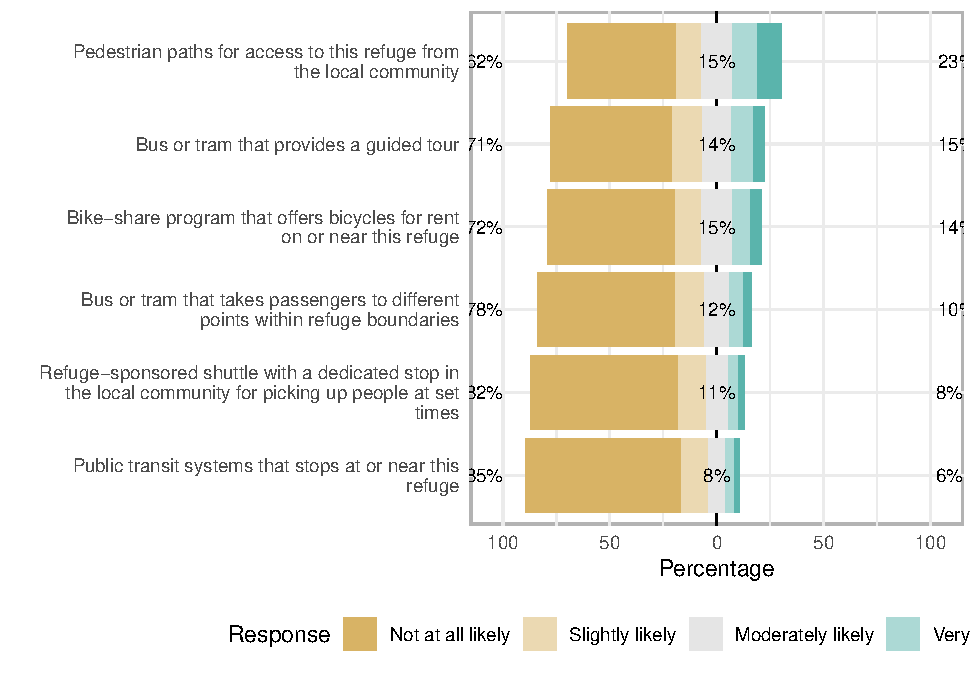
\includegraphics{nvs-report_files/figure-latex/alt-trans-1.pdf}
\caption{\label{fig:alt-trans}How likely visitors would be to use each
transportation option at this refuge if it were available in the
future.}
\end{figure}

\chapter{Visitor Spending in the Local Communities}\label{econ}

\BeginKnitrBlock{heading4}
Tourists tend to buy a range of goods and services while visiting an
area, such as a city or town located adjacent to a refuge. Major
expenditure categories include lodging, food, supplies, and gasoline.
Spending associated with refuge visitation can generate considerable
economic benefits for local communities. For example, more than 46.5
million visits were made to refuges in fiscal year 2011, and generated
\$2.4 billion in sales, more than 35,000 jobs, and \$792.7 million in
employment income in regional economies \citep{carver2013}. Information
on the amount and types of visitor expenditures in relation to
particular recreation activities (e.g., hunting, fishing, wildlife
observation) has further illustrated the economic importance of
recreation \citep{USFWS2018}, which are the primary reasons for which
visitors seek out refuges and related resources. Finally, visitor
expenditure information can be used to determine the potential economic
impact of proposed refuge management alternatives into the future.
\EndKnitrBlock{heading4}

\section*{Visitor Spending in the Local
Communities}\label{visitor-spending-in-the-local-communities}
\addcontentsline{toc}{section}{Visitor Spending in the Local
Communities}

Visitors that live within the local 50-mi area of a refuge typically
have different spending patterns than those that travel from longer
distances. During the two sampling periods, 62\% of surveyed visitors to
Dungeness National Wildlife Refuge indicated that they live within the
local 50-mi area while nonlocal visitors (30\%) stayed in the local
area, on average, for NA days. (tab:expendTable) shows summary
statistics for local and nonlocal visitor expenditures in the local
communities and at the refuge, with expenditures reported on a per
person per day basis. During the two sampling periods, nonlocal visitors
(\emph{n} = 30) spent an average of \$140.17 per person per day and
local visitors spent an average of \$105.91 per person per day in the
local area. It is important to note that summary statistics based on a
small sample size (n \textless{} 30) may not provide a reliable
representation of that population. Several factors should be considered
when estimating the economic importance of refuge-visitor spending in
the local communities. These factors include the amount of time spent at
the refuge, influence of the refuge on the visitors' decision to take
this trip, and the representativeness of primary activities of the
sample of surveyed visitors compared to the general population.
Controlling for these factors is beyond the scope of the summary
statistics presented in this report.

Table: \label{tab:spend-table}

\begin{tabular}{lcrrrrr|lcrrrrr|lcrrrrr|lcrrrrr|lcrrrrr|lcrrrrr|lcrrrrr}
\hline
Visitors & n & Median & Mean & SD & Min & Max\\
\hline
2 & 0 & NA & NaN & NA & NA & NA\\
\hline
Local & 2140 & 12.50 & 105.91 & 1371.08 & 0 & 43783.00\\
\hline
Nonlocal & 1183 & 68.33 & 140.17 & 705.55 & 0 & 23166.67\\
\hline
\multicolumn{49}{l}{\textsuperscript{1} n = number of visitors who answered both locality and expenditure questions.}\\
\multicolumn{49}{l}{\textit{Note: }}\\
\multicolumn{49}{l}{For each respondent, reported expenditures were divided by the number of persons in their group that shared expenses in order to determine the spending per person per trip. This number was then divided by the number of days spent in the local area to determine the spending per person per day for each respondent. For respondents who reported spending less than one full day in the local community, trip length was set equal to one day. These visitor spending estimates are appropriate for the sampling periods selected by refuge staff (see [Table] for sampling period dates and (fig:primactFig) for the primary visitor activities in which people participated), and may not be representative of the total population of visitors to this refuge.}\\
\end{tabular}

\begin{figure}
\centering
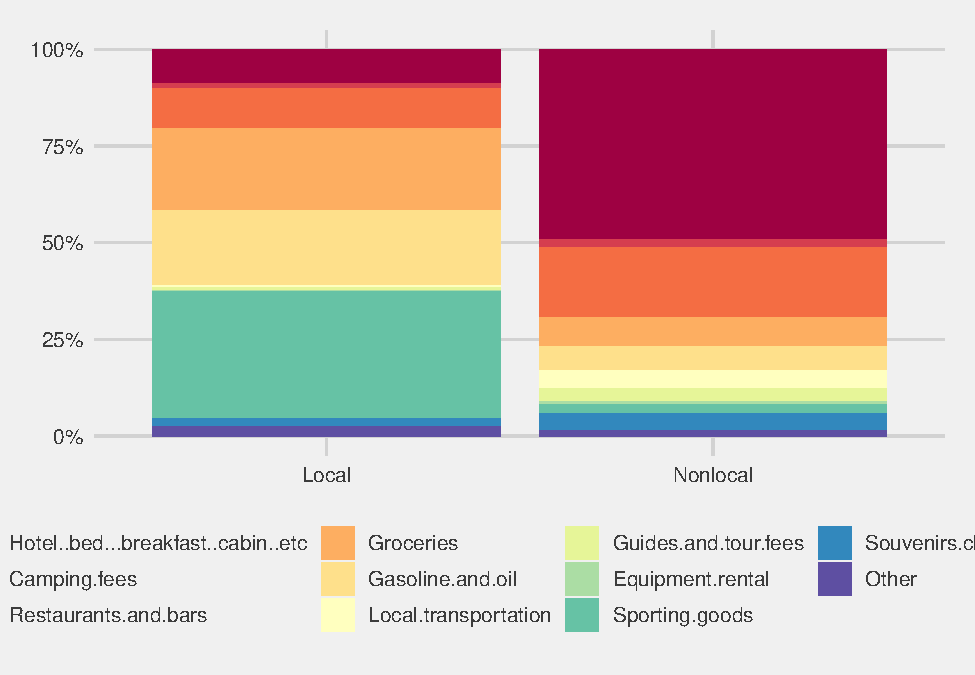
\includegraphics{nvs-report_files/figure-latex/unnamed-chunk-12-1.pdf}
\caption{\label{fig:unnamed-chunk-12}Total visitor expenditures in local
communities and at \texttt{r\ paste(params\$RefugeName)} expressed in
dollars per person per day}
\end{figure}

\chapter{Enhancing Future Visits to National Wildlife
Refuges}\label{futvis}

\section*{Forecasting Future Recreation Demand at This
Refuge}\label{forecasting-future-recreation-demand-at-this-refuge}
\addcontentsline{toc}{section}{Forecasting Future Recreation Demand at
This Refuge}

\BeginKnitrBlock{heading4}
Gaining a sense of what would encourage visitors to return (or what may
prevent them from returning) would be useful information for managers,
planners, and visitor services personnel. For example, some visitors may
prefer increased infrastructure, while others may want more access to
opportunities on the refuge. However, any management action aimed at
increasing recreation participation should be considered in relation to
possible effects on different visitor groups. For example, visitors may
report that more infrastructure would lead to increased participation in
a particular primary activity (e.g., birdwatching, fishing), but that
particular increased participation could also result in others feeling
crowded, subsequently reducing their participation. Thus, results in
this section should be considered as part of a network of potential
decisions that could affect different visitor groups disproportionally
if not carefully considered in full.
\EndKnitrBlock{heading4}

\section*{Visitor Programs}\label{visitor-programs}
\addcontentsline{toc}{section}{Visitor Programs}

\BeginKnitrBlock{heading4}
Offering programming that is equitable to various groups of visitors at
refuges, whether located in urban areas or elsewhere, will help to build
a stronger conservation constituency into the future \citep{USFWS2014}.
Creation and administration of different types of programs can encourage
people to continue visiting the refuge, and further build relationships
and encourage visitation among new audiences. These opportunities can
focus a variety of interests and topics ranging from skill-building,
specific youth programs, family-based or multi-generational programs, or
showcasing local or unique culture. Programs that focus on the interests
of these varied audiences in order to foster stronger connections to the
refuge and its resources may ultimately help to enhance conservation
goals.
\EndKnitrBlock{heading4}

\chapter{Conclusion}\label{concl}

These individual refuge results provide a summary of trip
characteristics and experiences of a sample of visitors to Dungeness
National Wildlife Refuge during 2018 and are intended to inform
decision-making efforts related to visitor services and transportation
at this refuge. Additionally, the results from this survey can be used
to inform planning efforts, such as a refuge's Comprehensive
Conservation Plan. With an understanding of visitors' trip and activity
characteristics, and visitor-satisfaction ratings with existing
offerings, refuge managers are able to make informed decisions about
possible modifications (whether a reduction or enhancement) to visitor
facilities, services, or recreational opportunities. This information
can help managers gauge demand for refuge opportunities and inform both
implementation and communication strategies. Similarly, an awareness of
visitors' satisfaction ratings with various refuge offerings can help
determine if potential areas of concern need to be investigated further.
As another example of the utility of these results, community relations
may be improved or bolstered through an understanding of the value of
the refuge to visitors, whether that value is attributed to an
appreciation of the refuge's offerings, enjoyment of its recreational
activities, or spending contributions of nonlocal visitors to the local
economy. Such data about visitors and their experiences, in conjunction
with an understanding of biophysical data on the refuge and its
resources, can ensure that management decisions are consistent with the
Refuge System mission while fostering a continued public interest in
these special places.

More information about the national visitor survey, including reports
for all participating refuges, are available at
go.osu.edu/refugereports.

More information regarding the Service's Human Dimensions Branch can be
found at
\url{https://www.fws.gov/Refuges/NaturalResourcePC/humanDimensions.html}.

\appendix


\chapter*{Appendix A. Project
Methods}\label{appendix-a.-project-methods}
\addcontentsline{toc}{chapter}{Appendix A. Project Methods}

\section*{Selecting Participating
Refuges}\label{selecting-participating-refuges}
\addcontentsline{toc}{section}{Selecting Participating Refuges}

The national visitor survey was conducted from March 2018 to April 2019
on 37 refuges across the Refuge System (tab:refuge-list). Each refuge
was selected for participation by regional office Visitor Services
Chiefs.

\begin{longtable}[]{@{}l@{}}
\caption{\label{tab:refuge-list}}\tabularnewline
\toprule
\begin{minipage}[b]{0.05\columnwidth}\raggedright\strut
\textbf{Refuges}\strut
\end{minipage}\tabularnewline
\midrule
\endfirsthead
\toprule
\begin{minipage}[b]{0.05\columnwidth}\raggedright\strut
\textbf{Refuges}\strut
\end{minipage}\tabularnewline
\midrule
\endhead
\begin{minipage}[t]{0.05\columnwidth}\raggedright\strut
\textbf{Pacific Region (R1)}\strut
\end{minipage}\tabularnewline
\begin{minipage}[t]{0.05\columnwidth}\raggedright\strut
Billy Frank Jr. Nisqually NWR (WA)Dungeness NWR (WA)Guam NWR (GU)Hanalei
NWR (HI)Kilauea Point NWR (HI)Ridgefield NWR (WA)Steigerwald Lake NWR
(WA)Tualatin River NWR (OR)\strut
\end{minipage}\tabularnewline
\begin{minipage}[t]{0.05\columnwidth}\raggedright\strut
\textbf{Southwest Region (R2)}\strut
\end{minipage}\tabularnewline
\begin{minipage}[t]{0.05\columnwidth}\raggedright\strut
Balcones Canyonlands NWR (TX) Hagerman NWR (TX)\strut
\end{minipage}\tabularnewline
\begin{minipage}[t]{0.05\columnwidth}\raggedright\strut
\textbf{Midwest Region (R3)}\strut
\end{minipage}\tabularnewline
\begin{minipage}[t]{0.05\columnwidth}\raggedright\strut
Crab Orchard NWR (IL) Loess Bluffs NWR (MO) Ottawa NWR (OH) Sherburne
NWR (MN) Shiawassee NWR (MI)\strut
\end{minipage}\tabularnewline
\begin{minipage}[t]{0.05\columnwidth}\raggedright\strut
\textbf{Southeast Region (R4)}\strut
\end{minipage}\tabularnewline
\begin{minipage}[t]{0.05\columnwidth}\raggedright\strut
A.R.M. Loxahatchee NWR (FL) Bayou Sauvage NWR (LA) Big Branch Marsh NWR
(LA) Cache River NWR (AR) J.N. Ding Darling NWR (FL) Okefenokee NWR (GA)
Pinckney Island NWR (SC) Sam D. Hamilton Noxubee NWR (MS) Tennessee NWR
(TN)\strut
\end{minipage}\tabularnewline
\begin{minipage}[t]{0.05\columnwidth}\raggedright\strut
\textbf{Northeast Region (R5)}\strut
\end{minipage}\tabularnewline
\begin{minipage}[t]{0.05\columnwidth}\raggedright\strut
Blackwater NWR (MD) Canaan Valley NWR (WV) Great Meadows NWR (MA) John
Heinz NWR at Tinicum (PA) Ohio River Islands NWR (PA) Prime Hook NWR
(DE) Sachuest Point NWR (RI)\strut
\end{minipage}\tabularnewline
\begin{minipage}[t]{0.05\columnwidth}\raggedright\strut
\textbf{Mountain-Prairie Region (R6)}\strut
\end{minipage}\tabularnewline
\begin{minipage}[t]{0.05\columnwidth}\raggedright\strut
Kirwin NWR (KS) Rainwater Basin WMD (NE) Sullys Hill National Game
Preserve (ND)\strut
\end{minipage}\tabularnewline
\begin{minipage}[t]{0.05\columnwidth}\raggedright\strut
\textbf{Alaska Region (R7)}\strut
\end{minipage}\tabularnewline
\begin{minipage}[t]{0.05\columnwidth}\raggedright\strut
None in 2018\strut
\end{minipage}\tabularnewline
\begin{minipage}[t]{0.05\columnwidth}\raggedright\strut
\textbf{Pacific Southwest Region (R8)}\strut
\end{minipage}\tabularnewline
\begin{minipage}[t]{0.05\columnwidth}\raggedright\strut
Desert NWR (NV) San Diego NWR (CA) San Diego Bay NWR (CA)\strut
\end{minipage}\tabularnewline
\bottomrule
\end{longtable}

\section*{Developing the Survey
Instrument}\label{developing-the-survey-instrument}
\addcontentsline{toc}{section}{Developing the Survey Instrument}

Researchers at OSU developed the survey in consultation with the Service
Headquarters Office, managers, planners, and visitor services
professionals. The survey was peer-reviewed by academic and government
researchers. The survey and associated methodology were approved by the
Office of Management and Budget (OMB control \#: 0596-0236; expiration
date: 11/30/2020).

\section*{Contacting Visitors}\label{contacting-visitors-1}
\addcontentsline{toc}{section}{Contacting Visitors}

Refuge staff identified two separate 14-day sampling periods, and one or
more locations at which to sample, that best reflected the diversity of
use and specific visitation patterns of each participating refuge. A
standardized sampling schedule was created for all refuges that included
eight randomly selected sampling shifts during each of the two sampling
periods. Sampling shifts were four (hr) time bands, stratified across AM
and PM as well as weekend and weekdays. In coordination with refuge
staff, any necessary customizations were made to the standardized
schedule to accommodate the identified sampling locations and to address
specific spatial and temporal patterns of visitation.

Twenty visitors (18 years of age or older) per sampling shift were
systematically selected, for a total of 400 willing participants per
refuge (or 200 per sampling period) to ensure an adequate sample of
completed surveys. When necessary, shifts were moved, added, or extended
to alleviate logistical limitations (for example, weather or low
visitation at a particular site) in an effort to reach target numbers.

American Conservation Experience Interns and/or USFWS Human Dimensions
staff (survey recruiters) contacted visitors onsite following a protocol
provided by OSU that was designed to obtain a representative sample.
Instructions included contacting visitors across the entire sampling
shift (for example, every nth visitor for dense visitation, as often as
possible for sparse visitation) and contacting only one person per
group. Visitors were informed of the survey effort, given a token
incentive (for example, a small magnet or temporary tattoo), and asked
to participate. Willing participants provided their name, mailing
address, and preference for language (English or Spanish). Survey
recruiters were also instructed to record any refusals and then proceed
with the sampling protocol

All visitors that agreed onsite to fill out a survey received the same
sequence of correspondence. This approach allowed for an assessment of
visitors' likelihood of completing the survey by their preferred survey
mode \citep{sexton2011}. Researchers at OSU sent the following materials
to all visitors agreeing to participate who had not yet completed a
survey at the time of each mailing \citep{dillman2014}:

\begin{itemize}
\tightlist
\item
  A postcard mailed within 10 days of the initial onsite contact
  thanking visitors for agreeing to participate in the survey and
  inviting them to complete the survey online.
\item
  A packet mailed 14 days later consisting of a cover letter, survey,
  and postage paid envelope for returning a completed paper survey.
\item
  A reminder postcard mailed 14 days later.
\item
  A second packet mailed 7 days later consisting of another cover
  letter, survey, and postage paid envelope for returning a completed
  paper survey.
\end{itemize}

Each mailing included instructions for completing the survey online, so
visitors had an opportunity to complete an online survey with each
mailing. Those visitors indicating a preference for Spanish were sent
Spanish versions of all correspondence (including the survey). Online
survey data were exported and paper survey data were entered into
Microsoft Excel using a standardized survey codebook and data entry
procedure. All survey data were analyzed using \emph{Statistical Package
for the Social Sciences} (SPSS, v.23) and R software\footnote{Any use of
  trade, firm, or product names is for descriptive purposes only and
  does not imply endorsement by the U.S. Government.}.

\section*{Interpreting the Results}\label{interpreting-the-results-1}
\addcontentsline{toc}{section}{Interpreting the Results}

The extent to which these results accurately represent the total
population of visitors to this refuge is dependent on the number of
visitors who completed the survey (sample size) and the ability of the
variation resulting from that sample to reflect the beliefs and
interests of different visitor user groups (Scheaffer and others, 1996).
The composition of the sample is dependent on the ability of the
standardized sampling protocol for this study to account for the spatial
and temporal patterns of visitor use unique to each refuge. Spatially,
the geographical layout and public-use infrastructure varies widely
across refuges. Some refuges can be accessed only through a single
entrance, while others have multiple unmonitored access points across
large expanses of land and water. As a result, the degree to which
sampling locations effectively captured spatial patterns of visitor use
will vary from refuge to refuge. Temporally, the two 14-day sampling
periods may not have effectively captured all of the predominant visitor
uses/activities on some refuges during the course of a year, which may
result in certain survey measures such as visitors' self-reported
``primary activity during their visit'' reflecting a seasonality bias.
Results contained within this report may not apply to visitors during
all times of the year or to visitors who did not visit the survey
locations.

In this report, visitors who responded to the survey are referred to
simply as ``visitors.'' However, when interpreting the results for
Dungeness National Wildlife Refuge, any potential spatial and temporal
sampling limitation specific to this refuge needs to be considered when
generalizing the results to the total population of visitors. For
example, a refuge that sampled during a special event (for example,
birding festival) held during the spring may have contacted a higher
percentage of visitors who traveled greater than 50 miles (mi) to get to
the refuge than the actual number of these people who would have visited
throughout the calendar year (that is, oversampling of nonlocals).
Another refuge may not have enough nonlocal visitors in the sample to
adequately represent the beliefs and opinions of that group type. If the
sample for a specific group type (for example, nonlocals, hunters,
visitors who paid a fee) is too low (\emph{n} \&lt; 30), a warning is
included in the text. Finally, the term ``this visit'' is used to
reference the visit during which people were contacted to participate in
the survey.

\section*{Non-Response Bias}\label{non-response-bias}
\addcontentsline{toc}{section}{Non-Response Bias}

Non-response bias is the bias that results when respondents differ in
meaningful ways from nonrespondents. Non-response bias affects the
ability to generalize survey results, to some degree and in some ways,
from the sample to the study's target population
\citep[\citet{salant1994}]{dillman2014}. If non-respondents are found to
differ from respondents in meaningful ways, care should be taken when
interpreting survey responses, as they may overrepresent some segments
of the target population to some degree, and may under-represent other
segments of the population to some degree.

To check for non-response bias, this study used answers to three
non-response bias questions and three observable characteristics of the
contacted visitor to compare respondents with nonrespondents. The
following questions and observations were used for evaluation of
non-response bias: - What is your primary activity at the refuge today?
- Do you live within 50 miles of this refuge? - What year were you born?

In addition to the three non-response bias questions, the following
three characteristics were observed and recorded: - Gender of the person
in the group who was first contacted by the survey recruiter - Number of
adults (18 years and older) in the group - Number of children (under 18
years) in the group

Ideally, responses or observed estimates for non-response bias variables
should be collected from all respondents and non-respondents. The
collection of information from all contacted individuals provides the
best comparison of characteristics between the respondent and
non-respondent populations. More practically, a majority of responses or
observed estimates must be present to adequately characterize both the
respondent and non-respondent populations. In this study, 70\% was
identified as the minimum percentage of valid values for non-response
variables needed for both respondent and non-respondent populations in
order to adequately characterize the populations on a given non-response
variable. All non-response variables met the minimum for 70\% valid
values among respondents and/or non-respondents \ref{tab:nonresponse}.
Correspondingly, all variables were used for non-response bias analysis.

\begin{longtable}[]{@{}lll@{}}
\caption{\label{tab:nonresponse} Number and percentage of respondents and
non-respondents with valid values for nonresponse
variable}\tabularnewline
\toprule
\textbf{Variable} & \textbf{Respondents} &
\textbf{Non-Respondents}\tabularnewline
\midrule
\endfirsthead
\toprule
\textbf{Variable} & \textbf{Respondents} &
\textbf{Non-Respondents}\tabularnewline
\midrule
\endhead
Gender & x & y\tabularnewline
Number of Adults & x & y\tabularnewline
Number of Children & x & y\tabularnewline
\bottomrule
\end{longtable}

\chapter*{Appendix B: Survey Frequencies for Dungeness National Wildlife
Refuge}\label{AppendixB}
\addcontentsline{toc}{chapter}{Appendix B: Survey Frequencies for
Dungeness National Wildlife Refuge}

\section*{Overall Satisfaction}\label{overall-satisfaction-1}
\addcontentsline{toc}{section}{Overall Satisfaction}

\section*{Recreational
Opportunities}\label{recreational-opportunities-1}
\addcontentsline{toc}{section}{Recreational Opportunities}

\subsection*{Importance of Recreational
Opportunities}\label{importance-of-recreational-opportunities}
\addcontentsline{toc}{subsection}{Importance of Recreational
Opportunities}

\begin{figure}
\centering
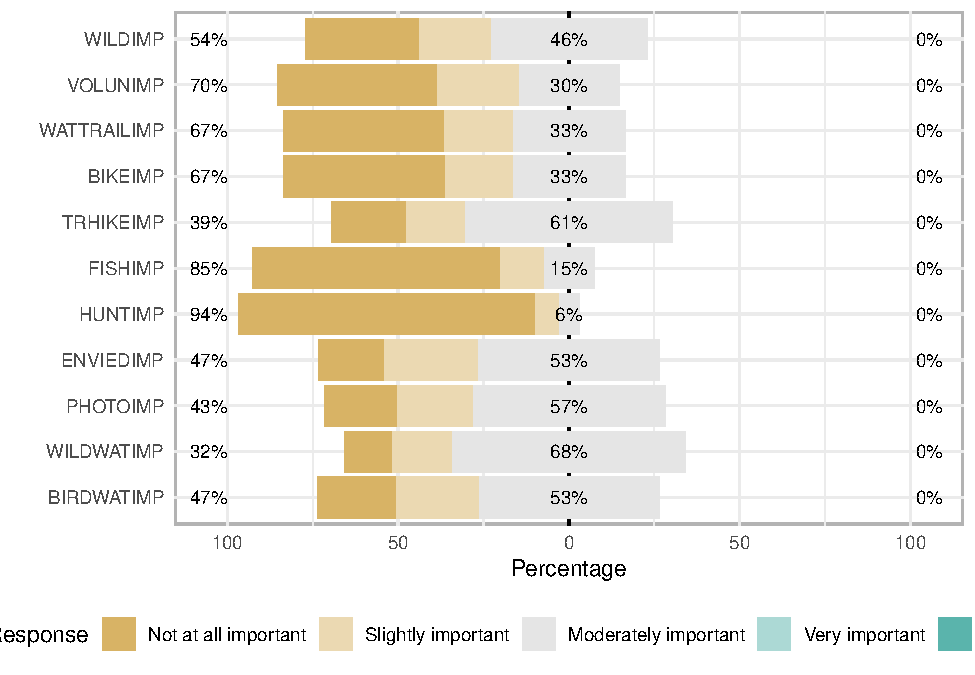
\includegraphics{nvs-report_files/figure-latex/recImp-1.pdf}
\caption{\label{fig:recImp}How important are the recreation opportunities?}
\end{figure}

\subsection*{Satisfaction with Recreational
Opportunities}\label{satisfaction-with-recreational-opportunities}
\addcontentsline{toc}{subsection}{Satisfaction with Recreational
Opportunities}

\begin{figure}
\centering
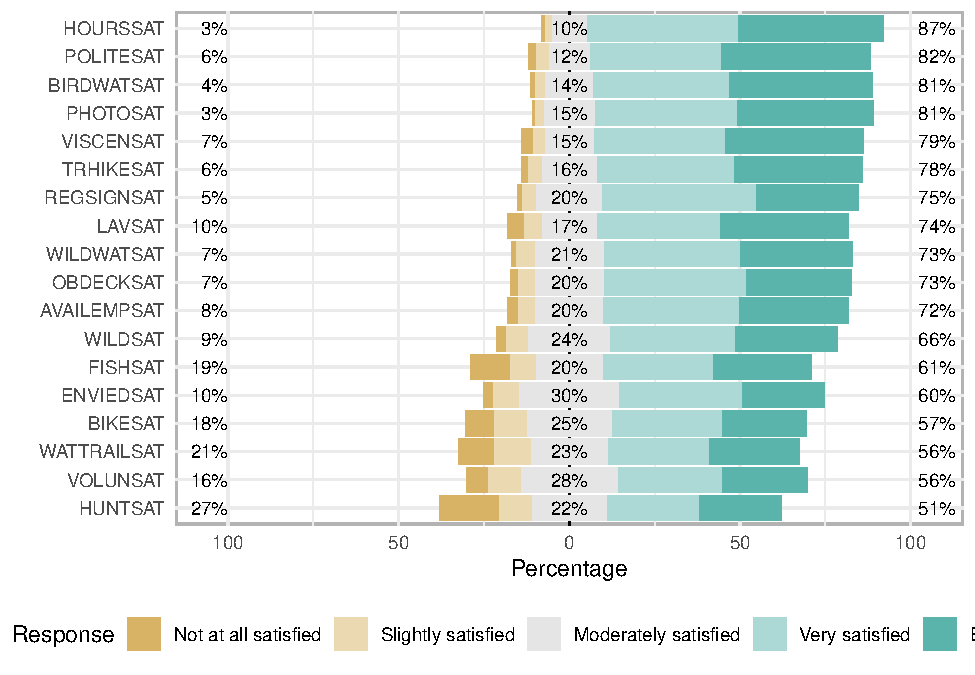
\includegraphics{nvs-report_files/figure-latex/recSat-1.pdf}
\caption{\label{fig:recSat}How satisfied are you with the recreation
opportunities?}
\end{figure}

\section*{Services and Facilities}\label{services-and-facilities-1}
\addcontentsline{toc}{section}{Services and Facilities}

Positive experiences are driven by first impressions of refuge
facilities and people.

\subsection*{Importance of Facilities and
Services}\label{importance-of-facilities-and-services}
\addcontentsline{toc}{subsection}{Importance of Facilities and Services}

servicesImpTitle
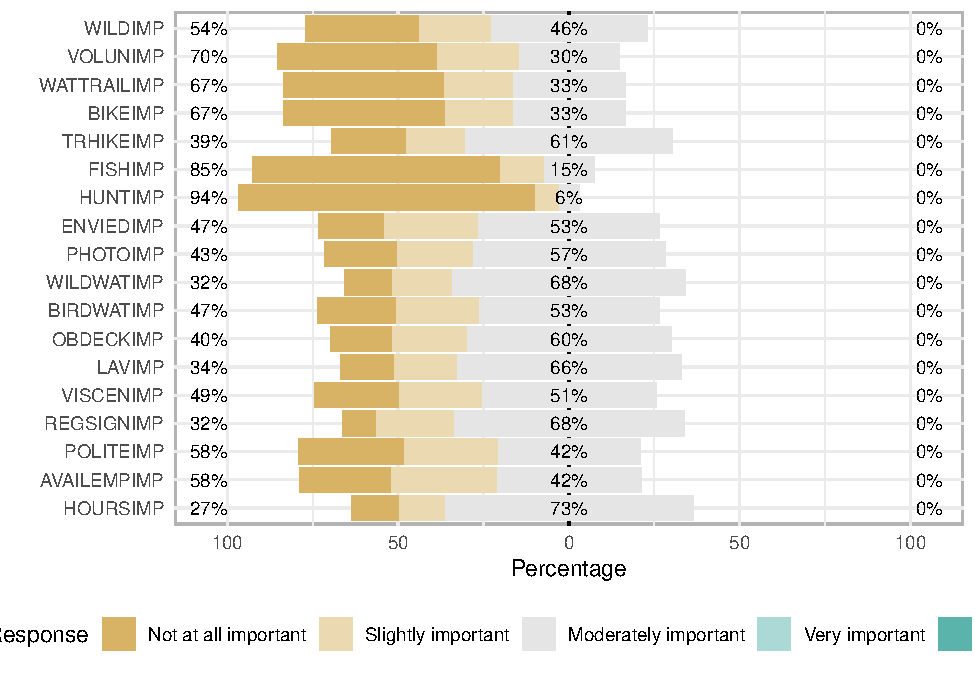
\includegraphics{nvs-report_files/figure-latex/servicesImp-1.pdf}

\subsection*{Satisfaction with Facilities and
Services}\label{satisfaction-with-facilities-and-services}
\addcontentsline{toc}{subsection}{Satisfaction with Facilities and
Services}

\begin{figure}
\centering
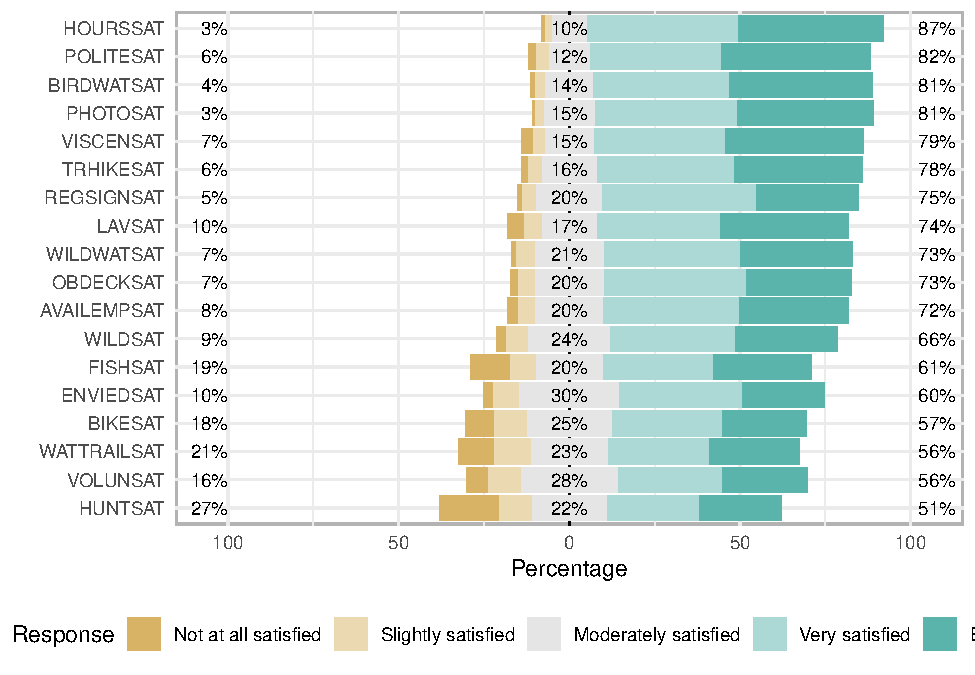
\includegraphics{nvs-report_files/figure-latex/servSatPlot-1.pdf}
\caption{\label{fig:servSatPlot}Rate how satisfied you are with the way this
refuge is managing each feature}
\end{figure}

\section*{Feeling Safe and Welcome}\label{feeling-safe-and-welcome-1}
\addcontentsline{toc}{section}{Feeling Safe and Welcome}

safeTitle
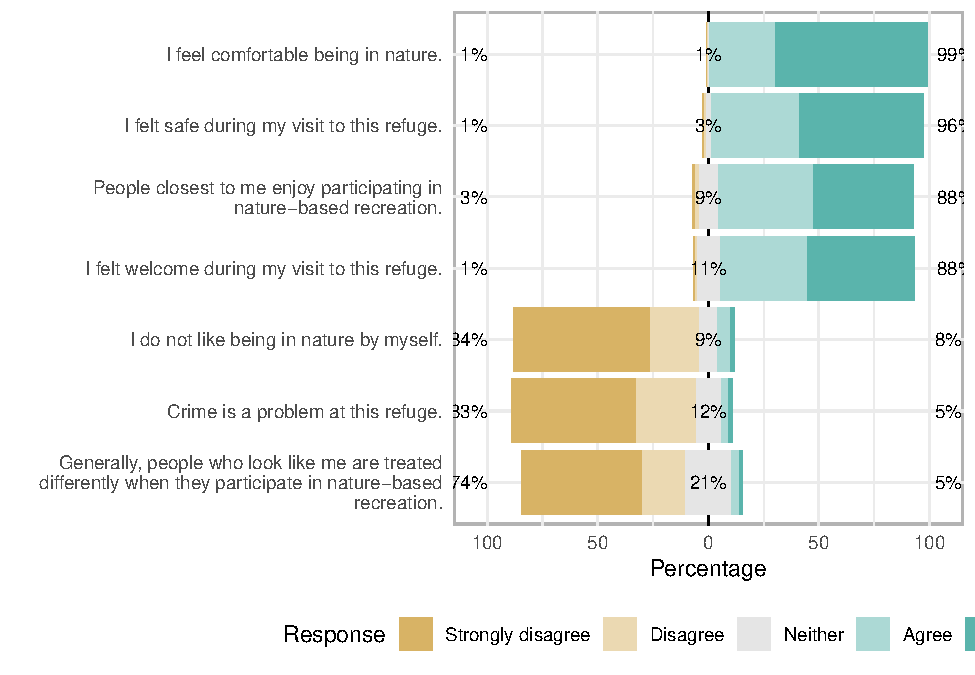
\includegraphics{nvs-report_files/figure-latex/unnamed-chunk-17-1.pdf}

\bibliography{book.bib,packages.bib}


\end{document}
